%\documentclass[9pt,twocolumn,twoside]{pnas-new}
\documentclass[twocolumn,twoside]{article}
%\documentclass[twocolumn,showpacs,%
%  nofootinbib,aps,superscriptaddress,%
%  eqsecnum,prd,notitlepage,showkeys,9pt]{article}

%TODO remove PNAS instructions 
% SWITCH back to bvect

% Use the lineno option to display guide line numbers if required.
% Note that the use of elements such as single-column equations
% may affect the guide line number alignment. 

%\templatetype{pnasresearcharticle} % Choose template 
% {pnasresearcharticle} = Template for a two-column research article
% {pnasmathematics} = Template for a one-column mathematics article
% {pnasinvited} = Template for a PNAS invited submission

%% ------------------------------------------------------ %%
%% ------------ Additional Packages/Commands ------------ %%
%% ------------------------------------------------------ %%
\usepackage[T1]{fontenc}
\usepackage[utf8]{inputenc}
\usepackage{newunicodechar}
\usepackage[margin=0.7in]{geometry}
\usepackage{textcomp}
\usepackage{gensymb}
\usepackage{amssymb}
\usepackage{mathtools}
\usepackage{mathrsfs}
\usepackage{eucal}
\usepackage{units}
\usepackage{siunitx}
\usepackage{color}
\usepackage{bm} % for bold vectors
\usepackage{upgreek} % for bold greek-letter vectors
%\usepackage{algorithmicx}
\usepackage{algorithm,algorithmic,setspace} % http://ctan.org/pkg/algorithms
%\usepackage[noend]{algpseudocode} % http://ctan.org/pkg/algorithmicx
\usepackage[section]{placeins}
\usepackage{afterpage} % for clearing page after figure
\usepackage{titling} % for title
\usepackage{caption} % for caption in minipage environment
\usepackage{authblk} % for affiliations
\usepackage{parskip} % Removes indentation from paragraphs
%\usepackage[bottom]{footmisc}
%\raggedbottom % allow paragraphs to end before page bottom

% Remove algorithm number label, as there is only one
%\captionsetup[algorithm]{labelformat=empty}

\newcommand{\conj}[1]{\overline{#1}}
%\newcommand{\Mxy}{\widetilde{M}_{xy}}
%\newcommand{\Mxy}{\widetilde{M}}
\newcommand{\Mxy}{\mathcal{M}}
\newcommand{\CDecay}{\Gamma}
\newcommand{\conv}{\ast}
\newcommand{\Lap}{\nabla^2}

%\newcommand{\vect[1]}{\vec{#1}} %vectors using arrows
\newcommand{\vect}[1]{\mathbf{#1}} %vectors using boldface
\newcommand{\bvect}[1]{\bm{#1}} % \mathbf doesn't work for greek/mathcal letters
%\newcommand{\bvect}[1]{#1} % looks better without bold

\newcommand{\matr}[1]{\mathbf{#1}} % matrix: undergraduate algebra version
%\newcommand{\matr}[1]{\bm{#1}}    % matrix: ISO complying version

%\newcommand{\tensor}[1]{\overleftrightarrow{\matr{#1}}} % for diffusion tensor
%\newcommand{\tensor}[1]{\overset{\text{\tiny$\leftrightarrow$}}{\matr{#1}}}
\newcommand{\tensor}[1]{\matr{#1}} % for diffusion tensor
%\def\tensor#1{\protect\@ontopof{#1}{\leftrightarrow}{1.15}\mathord{\box2}}

% for capital 'M' for molar
\DeclareSIUnit\Molar{\text{M}}

% Prevent inline equations from breaking over lines
\relpenalty=9999 %10000 means never, 9999 means almost never
\binoppenalty=9999

% Prevent over hyphenation of words across lines
\pretolerance=2000 %10000 means never, 9999 means almost never
\tolerance=2000 
\emergencystretch=10pt % maximum width of allowed extra space is 10pt

%% Begin added or changed by Alex Rauscher
\renewcommand{\floatpagefraction}{0.8} % so that pictures don't occupy 
                                       % an entire column
% changed CA\textsubscript{PEAK} to  $\text{CA}_{\text{PEAK}}$
%% End added by Alex Rauscher

% force figures to be at the top of the page, not float in the middle
\makeatletter
\setlength{\@fptop}{0pt}
\makeatother

%\DeclareUnicodeCharacter{01E7}{ǧ} % does NOT work; pdflatex halts
\newunicodechar{ǧ}{\u{g}} % not sure why, but this needs to be defined

% For a regular tilde...
\newcommand{\mytilde}{\raise.17ex\hbox{$\scriptstyle\mathtt{\sim}$}}
\newcommand{\myast}{\lower.17ex\hbox{*}}

%% ------------------------------------------------------ %%
%% ------------------------------------------------------ %%
%% ------------------------------------------------------ %%

%% ------------------------------------------------------ %%
%% --------------- Shorthands for Results --------------- %%
%% ------------------------------------------------------ %%

% SE perf orientation best fit parameters
\newcommand{\Lbest}{4} % number of anisotropic vessels
\newcommand{\CAbest}{\SI{6.39}{\milli\Molar}} % number of anisotropic vessels
\newcommand{\BVFbest}{2.52\%} % BVF percent
\newcommand{\iBVFbest}{1.18\%} % isotropic BVF percent
\newcommand{\aBVFbest}{1.34\%} % anisotropic BVF percent
\newcommand{\iRBVFbest}{46.8\%} % isotropic BVF percent
\newcommand{\aRBVFbest}{53.2\%} % anisotropic BVF percent

%Vessel sizes (for 13.7um minor vessels)
% N  R [um]
% 1  189.7268
% 2  129.3912
% 3  105.2080
% 4  91.8303
% 5  81.5069
% 6  73.6895
% 7  68.3088
% 8  61.4429
% 9  58.3809

%Vessel sizes (for 7um minor vessels)
\newcommand{\RMAJORone}{\SI{217.6}{\micro\meter}}   % radius for 1 major
\newcommand{\RMAJORtwo}{\SI{135.6}{\micro\meter}}   % radius for 2 major
\newcommand{\RMAJORthree}{\SI{110.3}{\micro\meter}} % radius for 3 major
\newcommand{\RMAJORfour}{\SI{96.9}{\micro\meter}}   % radius for 4 major
\newcommand{\RMAJORfive}{\SI{84.4}{\micro\meter}}   % radius for 5 major
\newcommand{\RMAJORsix}{\SI{72.8}{\micro\meter}}    % radius for 6 major
\newcommand{\RMAJORseven}{\SI{68.4}{\micro\meter}}  % radius for 7 major
\newcommand{\RMAJOReight}{\SI{63.7}{\micro\meter}}  % radius for 8 major
\newcommand{\RMAJORnine}{\SI{57.4}{\micro\meter}}   % radius for 9 major

\newcommand{\RMAJORbest}{\RMAJORfour} % best result was L=4


%% ------------------------------------------------------ %%
%% ------------------------------------------------------ %%
%% ------------------------------------------------------ %%

\setlength{\droptitle}{-0.8cm}
\title{Fiber tract orientation dependent white matter signal in functional MRI}

% Use letters for affiliations, numbers to show equal authorship (if applicable) and to indicate the corresponding author
%\author{Jonathan Doucette$^{1,1}$, Luxi Wei$^{1,3}$, 
%Enedino Hernández-Torres$^{1,4}$, Christian Kames$^{1,1}$,\\
%Nils Daniel Forkert$^{5}$, Rasmus Aamand$^{6}$, 
%Torben E. Lund$^{6}$, Brian Hansen$^{6}$ \& 
%Alexander Rauscher$^{1,3,4}$}
\author[a,b,\textasteriskcentered]{Jonathan Doucette}
\author[a,c]{Luxi Wei}
\author[a,d]{Enedino Hernández-Torres}
\author[a,b]{Christian Kames}
\author[e]{Nils Daniel Forkert}
\author[f]{Rasmus Aamand}
\author[f]{Torben E. Lund}
\author[f]{Brian Hansen}
\author[a,b,d]{Alexander Rauscher}

\affil[a]{UBC MRI Research Centre, University of British Columbia,
  2221 Wesbrook Mall, Vancouver, BC, Canada.}%, V6T 2B5.}

\affil[b]{Department of Physics and Astronomy, University of British
  Columbia, 6224 Agricultural Road, Hennings Building, Room 325,
  Vancouver, BC, Canada.}%, V6T 1Z1.}

\affil[c]{Department of Medical Biophysics, University of Toronto, Toronto, ON, Canada}

\affil[d]{Department of Pediatrics, University of British Columbia
  Faculty of Medicine, Rm 2D19, 4480 Oak Street, BC Children's
  Hospital, Vancouver, BC, Canada.}%, V6H 3V4.}

\affil[e]{Department of Radiology and Hotchkiss Brain Institute,
  University of Calgary, Calgary, AB, Canada.}

% spacing after last affiliation before date:
\affil[f]{Center of Functionally Integrative Neuroscience (CFIN) and
  MINDLab, Department of Clinical Medicine, Aarhus University
  Hospital, Nørrebrogade 44, Building 10G, 5th floor, 8000 Aarhus C,
  Denmark.\vspace{0.5cm}}

% spacing after last affiliation before date:
%\affil[*]{Corresponding Author\vspace{0.5cm}}

\date{\today}
\setcounter{Maxaffil}{0}
\renewcommand\Affilfont{\itshape\small}

% Please give the surname of the lead author for the running footer
%\leadauthor{Doucette} 

% Please add here a significance statement to explain the relevance of
% your work MUST BE <= 120 WORDS (currently 109, Aug. 10, 2017)
%\significancestatement{Blood flow, volume, and oxygenation are of
%  fundamental importance for brain physiology and can be probed with
%  magnetic resonance imaging (MRI). However, the details of how
%  structurally isotropic and anisotropic components of the cerebral
%  vascular tree affect the measurements of these parameters are poorly
%  understood. Here, we show that in the brain's white matter, a
%  considerable portion of the blood resides in vessels that run in
%  parallel with the white matter tracts. We demonstrate that this
%  anisotropy has a profound impact on dynamic susceptibility contrast
%  and functional MRI by causing a strong tissue orientation dependence
%  of the MRI signal, with important implications for MRI of brain
%  function and perfusion.}

% -------------------------------- %TODO ---------------------------------%
%	Nature Communications:
%		You must include a statement that specifies the
%		individual contributions of each co-author. For example: "A.P.M.
%		‘contributed’ Y and Z; B.T.R. ‘contributed’ Y,” etc.
%		See our authorship policies for more details
% -------------------------------- %TODO ---------------------------------%
% Please include corresponding author, author contribution and author declaration information
%\authorcontributions{JD: data analysis, numerical simulations,
%  interpretation of results, writing of manuscript; LW: numerical
%  simulations; EHT: data analysis; CK: numerical simulations; RO, TEL,
%  and BH: data acquisition and interpretation of results; AR: idea,
%  interpretation of results, writing of manuscript; all authors
%  contributed to the editing of the manuscript }
%\authordeclaration{The authors have no conflicts of interest to
%  declare.}
%\equalauthors{\textsuperscript{1}A.O.(Author One) and A.T. (Author Two) contributed equally to this work (remove if not applicable).}
%\correspondingauthor{\textsuperscript{2}To whom correspondence should
%  be addressed. E-mail: jonathan.doucette@alumni.ubc.ca}

% Keywords are not mandatory, but authors are strongly encouraged to
% provide them. If provided, please include two to five keywords,
% separated by the pipe symbol, e.g:
%\keywords{Cerebral perfusion $|$ White matter $|$ Blood vessels $|$
% Diffusion $|$ Functional MRI}

%\dates{This manuscript was compiled on \today}
%\doi{\url{www.pnas.org/cgi/doi/10.1073/pnas.XXXXXXXXXX}}

\begin{document}
% Optional adjustment to line up main text (after abstract) of first page with line numbers, when using both lineno and twocolumn options.
% You should only change this length when you've finalised the article contents.
%\verticaladjustment{-2pt}

\maketitle
%\thispagestyle{firststyle}
%\ifthenelse{\boolean{shortarticle}}{\ifthenelse{\boolean{singlecolumn}}{\abscontentformatted}{\abscontent}}{}

%% SUGGESTED FORMAT:
%  -Title
%  -Author
%  -Affiliation
%  -Keywords
%  -Abstract
%  -Significance Statement
%  -Introduction
%  -Results
%  -Discussion
%  -Materials and methods
%  -Acknowledgments
%  -References
%% NOTE: Other orders and headings are permitted

% I would vote for methods before results, if that's possible. 

%TODO Abstract is bold in Nature, and should be approx 150 words
% (currently, ~200. probably OK for initial submission)
\textbf{Blood vessel related magnetic resonance imaging (MRI) contrast
  provides a window into the brain’s metabolism and function. Here, we
  investigate the blood oxygenation level dependent (BOLD) MRI signal
  based on first principles derived from dynamic susceptibility
  contrast (DSC) MRI, diffusion tensor imaging (DTI), and theoretical
  considerations. We present a rapid numerical framework for the
  exploration of the isotropic and anisotropic components of the
  vascular tree and show that half of the white matter vascular volume
  is comprised of vessels running in parallel with white matter fibre
  tracts. The white matter blood volume corresponding to the best fit
  to the experimental data was 2.52\%, which is very close to the PET
  gold standard of 2.6\%. We show that the anisotropy of the brain's
  vascular architecture causes a strong tissue orientation dependence
  of the DSC MRI signal, with an apparent perfusion that is 20\%
  larger in fibres perpendicular to the main magnetic field compared
  to parallel fibres. We then performed forward calculations of the
  BOLD signal for 3 and 7 Tesla and show that the gradient echo BOLD
  signal is twice as large in white matter tracts perpendicular to the
  main magnetic field compared to tracts parallel to the main magnetic
  field. For the spin echo BOLD signal, the orientation effect is
  about 20\%. These findings have far reaching consequences for the
  interpretation of the existing literature on both functional and DSC
  MRI, as well as the conduction of future experiments using these
  techniques. The presented approach of fitting a vascular model to
  raw perfusion MRI data provides a new avenue for the measurement of
  global white matter blood volume.
}
%Corresponding author footer
{\let\thefootnote\relax\footnote{{*Corresponding author: jdoucette@phas.ubc.ca}}}
%{\let\thefootnote\relax\footnote{{\textsuperscript{†}e-mail: jdoucette@phas.ubc.ca}}}

%% INTRODUCTION (don't add section title)
The distribution of blood in the human brain is regulated
via a specialized vascular network. Although the brain comprises only
2\% of the total body mass, it receives 15\% of the cardiac
output~\cite{bouma_relationship_1990}. Cerebral blood flow (CBF),
volume (CBV), and oxygenation are, thus, essential parameters of
brain physiology and stable levels are required to maintain brain
function. MRI is able to probe these parameters, usually via changes
in the magnetic properties of the vascular system, to which the MRI
signal is exquisitely sensitive. In DSC MRI, a paramagnetic contrast
agent (CA) is administered intravenously during the repeated
acquisition of a rapid imaging technique~\cite{ostergaard_high_1996-1,
  ostergaard_high_1996}. BOLD fMRI uses changes in blood oxygenation
for the detection of neural activity~\cite{ogawa1990brain,ogawa1992}.
The vast majority of fMRI studies focus on the brain's gray matter,
but there are also reports on fMRI in white
matter~\cite{Gawryluk2014,fabri2011topographical,fraser2012white}.
Very recently, a study in 176 subjects suggested functional
networks that are related to specific white matter (WM)
tracts~\cite{Peer2017}. The origin of the WM fMRI signal,
however, is unclear. Potential sources are astrocytic
activity~\cite{petzold2011,smith2002} and NO-producing
neurons~\cite{barbaresi2014}.  

Both DSC MRI and BOLD fMRI data can be acquired with gradient echo or
spin echo scans. In either case, the contrast mechanism is a change in
coherence due to the field inhomogeneities around the blood vessels,
which depend on CA concentration and blood oxygenation, and a change
in intravascular relaxation times. With decreasing blood oxygenation
or increasing CA concentration, the vessels become more paramagnetic
and the field inhomogeneities become
stronger~\cite{rauscher2005a,ogawa1990brain}, %TODO is this the right ogawa ref?
which results in an accelerated
loss of coherence. Analysis of fMRI and DSC scans usually assumes that
the vascular architecture within the voxel is spatially isotropic, and
therefore that the local orientation of the vasculature relative to
the main magnetic field plays no role. However, there is compelling
evidence that the vascular bed is not isotropic, particularly in white
matter. Postmortem images show many vessels running in parallel with
WM
tracts~\cite{nonaka_microvasculature_2003-1,nonaka_microvasculature_2003,
  okudera_micro-angiographical_1999}. Microscopic images of a rodent
model of ischemia~\cite{cavaglia_regional_2001}, and maps of
perivascular spaces in humans~\cite{cai_feasibility_2015} exhibit
anisotropy of the vascular architecture. In venography based on
susceptibility weighted imaging
(SWI)~\cite{deistung_susceptibility_2008,
  reichenbach_high-resolution_2001,denk_susceptibility_2010}, the
anisotropy of the vascular system can be readily appreciated in vivo.
Finally, and especially important for functional MRI, the orientation
of cortical tissue influences the strength of the BOLD
signal~\cite{gagnon_quantifying_2015}.

It has been recently shown that the gradient echo perfusion signal and
the maps of CBF and CBV derived therefrom show a strong dependence on
the local orientation of WM fibre
tracts~\cite{hernandez-torres_anisotropic_2016}.  Numerical
simulations of static spin dephasing that best fit the measured data
suggested that about half the blood volume is within larger
anisotropic vessels~\cite{hernandez-torres_anisotropic_2016}.

Gradient echo scans are usually used for fMRI and DSC experiments, due
to their high sensitivity to changes in blood oxygenation or CA
concentration. However, spin echo scans are also sensitive to the
presence of an intravascular CA or to changes in blood oxygenation
because the spins lose coherence when they diffuse in the magnetic
inhomogeneous environment created by the blood
vessels~\cite{boxerman_mr_1995}. Since smaller vessels produce
stronger field gradients, the spin echo signal is more sensitive to
small vessels than to large vessels. For this reason, spin echo fMRI
is more specific to the location and spatial extent of neural
activation~\cite{Uludag2009,Norris2012,uludag2017}. If the vascular
system is structurally isotropic, loss of coherence is
orientation-independent. With anistropic vascular architecture, on the
other hand, the loss of coherence should depend on tissue orientation
and give rise to orientation effects in MRI.

The anisotropy of the cerebral vasculature, in particular in WM,
raises several questions: How strongly do the DSC and BOLD signals
depend on the orientation of WM? How much blood resides in the
isotropic and anisotropic compartment of the vascular network, and
what is the role of vessel size? Finally, what are the implications of
vascular anisotropy for BOLD fMRI?

In this work, we investigate the vascular
architecture experimentally by combining spin echo DSC with diffusion
tensor imaging for the analysis of WM fibre orientation. We then fit a
model of the spin echo signal for fibre orientations between
\SI{0}{\degree} and \SI{90}{\degree} from which we extract isotropic
and anisotropic components of the vascular tree. These calculations
require the solution of the Bloch-Torrey equation, which describes the
spin echo signal in a magnetically inhomogeneous environment. Since we
fit vascular parameters to the orientation dependent DSC signal,
thousands of solutions of the Bloch-Torrey equation need to be
computed on a large anisotropic 3D grid. To do so in a computationally
feasible manner, we develop a framework that is based on the
equivalence of the Bloch-Torrey equation to the single-particle time
dependent Schrödinger equation. The vascular architecture that best
fits the observed DSC signal is then taken as the input for a forward
calculation of the BOLD signal at a range of echo times for both
gradient echo and spin echo fMRI at 3 and 7 Tesla.

%% MATERIALS AND METHODS
%\matmethods{%% BEGIN: MATERIALS AND METHODS
% 
% MOVED INTO THEORY/METHODS SECTION
%
%}%% END: MATERIALS AND METHODS

\section*{Materials and Methods}
\subsection*{Theoretical Considerations}

We first develop a numerical framework for the investigation of the
effect of field inhomogeneities on the DSC signal. The simulation
contains a small number of free parameters, which will be determined by
fitting the simulated DSC signal data to the corresponding
experimental data in a non-linear least squares fashion. These
parameters will then be used for a forward calculation of the BOLD
effect in WM.


%\subsection*{Perfusion Experiment}

The simulated DSC data is the change in transverse relaxation
$\Delta R_2$ that occurs due to the administration of the paramagnetic CA.
This change in $R_2$ can be computed by simulating the magnetization within    
a single WM voxel until an echo time TE, both with and without CA.
The resulting $\Delta R_2$ is given by
%
\begin{equation}\label{R2_Equation}
    \Delta R_2 = -\frac{1}{\text{TE}} \ln \Big( \frac{S}{S_0} \Big),
\end{equation}
%
where $S_0$ is the signal before the arrival of the CA, and $S$ is the
signal at the time point corresponding to peak
CA concentration~\cite{ostergaard_high_1996-1, ostergaard_high_1996}.
In order to investigate the effect of WM fibre tract orientation on the
resulting $\Delta R_2$ values, we define $\alpha$ to be the angle
between the main magnetic field and the WM fibre and allow $\alpha$ to
vary between \SI{0}{\degree} and \SI{90}{\degree} in the simulations.
The two major components of the simulations are
the generation of the geometry of
the problem for a given set of simulation parameters, and the
subsequent propagation of the magnetization through time.

The simulation takes place inside a single voxel of dimensions
$3\times 3\times \SI{3}{\milli\meter^3}$,
corresponding to the scan used to
acquire the data. Inside this voxel, we place an isotropic vascular
bed consisting of small blood vessels (\mytilde{}\SI{10}{\micro\meter}),
as well as anisotropic vasculature consisting of a variable number $L$
of large blood vessels (\mytilde{}\SI{100}{\micro\meter})
running in parallel with the $z$-axis. An example of this geometry
with $L=5$ anisotropic vessels is shown in
Figure~\ref{fig:geometry}. The orientation of the WM fibres is assumed
parallel to the anisotropic blood
vessels~\cite{nonaka_microvasculature_2003-1,nonaka_microvasculature_2003,okudera_micro-angiographical_1999,cavaglia_regional_2001,cai_feasibility_2015,deistung_susceptibility_2008},
and therefore the WM fibre is oriented in the $z$-direction as
well. The total amount of vasculature contained in the voxel is
determined by the blood volume fraction (BVF), a free parameter. The
isotropic vasculature is simulated as cylinders with uniformly random
orientation and position within the voxel,
% ---- 13.7um vessels ---- %
%with radii normally distributed with a mean of
%$\unit[13.7]{\mu m}$
%and a standard deviation of
%$\unit[2.1]{\mu m}$~\cite{jochimsen_whole-brain_2010}.
% ---- 7um vessels ---- %
with radii of \SI{7.0}{\micro\meter}~\cite{meier-ruge_stereological_1980}.
% --------------------- %
The total number of isotropic
vessels is determined by a second free parameter, the isotropic
relative blood volume fraction (iRBVF). The anisotropic vasculature is
simulated as uniformly spaced cylinders with axes parallel to the
$z$-direction. The radii of the anisotropic vessels are determined by
the anisotropic relative blood volume fraction (aRBVF), a constrained
parameter given by $\text{aRBVF} = 1 - \text{iRBVF}$.

The voxel may now be thought of as being separated into vasculature
and the surrounding tissue. In these regions, we prescribe different
values for the relaxation rate $R_2$ and for the magnetic
susceptibility $\chi$. Additionally, the value of both $R_2$ and
$\chi$ within the blood depends on the peak CA concentration
($\text{CA}_{\text{PEAK}}$), the third free parameter of the
simulation. The dependence of $R_2$ and $\chi$ on
$\text{CA}_{\text{PEAK}}$ is detailed in our previous study; see
equation 4 in~\cite{hernandez-torres_anisotropic_2016}. Since $\chi$
is non-constant within the voxel, local magnetic field inhomogeneities
are induced according to equation \ref{dB_local}
%
\begin{equation}\label{dB_local}
    \frac{\delta B(\vect{r})}{B_0} = G_{\alpha}(\vect{r}) \conv \delta \chi(\vect{r}),
\end{equation}
%
where $G_\alpha$ is the unit dipole kernel defined as
%
\begin{equation}\label{Dipole_Image}
    G_{\alpha}(\vect{r}) = \frac{1}{4\pi} \frac{3 \cos^2(\theta) - 1}{r^3}.
\end{equation}
%
This is the forward field calculation for the magnetic field by
convolution of the spatial magnetic susceptibility distribution with a
unit dipole~\cite{marques_using_2008}. The spherical radial distance
and polar angle $(r,\theta)$ in equation \ref{Dipole_Image} are
relative to the main magnetic field direction. In our simulations,
it is convenient to work in coordinates where the WM fibre is in the
$z$-direction, hence the subscript $\alpha$ on the dipole kernel. The
resulting local resonance frequency shift seen by the diffusing
protons is given by
%
\begin{equation}\label{dOmega}
    \delta \omega (\vect{r}) = \gamma \cdot \delta B(\vect{r}).
\end{equation}
%

In the experimental data, $\alpha$ was computed by taking the angle
between the main magnetic field direction and the principal diffusion
direction as measured with DTI. Each WM voxel was then sorted into
bins according to their $\alpha$-value. The bin widths were taken to
be 5$\degree$, resulting in 18 bins corresponding to angles from
2.5$\degree$ to 87.5$\degree$ in 5$\degree$ increments. In the
numerical simulations, $\alpha$ varies over these 18 angles in
order to match the experimental data. Cross sections of $\delta \omega$
in the $xy$\nobreakdash-plane for three different angles $\alpha$ are
shown in Figure~\ref{fig:geometry}.

Next, we consider the propagation of the magnetization through
time, which is described by the Bloch-Torrey equation~\cite{torrey_bloch_1956}
%
\begin{equation}\label{Bloch_Torrey_Full}
    \frac{d\vect{M}}{dt} = \gamma \vect{M} \times \vect{B} - 
    \bigg[ \frac{M_x}{T_2}, \frac{M_y}{T_2}, 
    \frac{M_z-M_0}{T_1} \bigg]^T + 
    \nabla \cdot \tensor{D} \nabla \vect{M}. 
\end{equation}
%
Accounting for diffusion in the presence of the $\alpha$-dependent
field inhomogeneities introduces $\alpha$-dependent
simulated $\Delta R_2$ values.

Since $\text{TE} \approx T_2 \ll T_1$, we neglect $T_1$ effects. We
assume isotropic diffusion by setting $\tensor{D} = D \tensor{I}$.
Additionally, we denote
\begin{equation}\label{Complex_Magnetization}
    \Mxy \coloneqq M_x + i M_y
\end{equation}
the complex transverse magnetization and
\begin{equation}\label{Complex_Decay_Rate}
    \CDecay(\vect{r}) \coloneqq  R_2(\vect{r}) + i \omega(\vect{r})
\end{equation}
the complex decay rate, where
$\omega(\vect{r}) = \omega_0 + \delta\omega(\vect{r})$
with
$\omega_0 = \gamma B_0$,
and
$R_2(\vect{r})$ is the piecewise constant $R_2$ value taking different 
values in tissue and in blood.
% -- Maybe don't need this sentence? -- %
%Herein, the term decay refers to the complex
%decay due to $\CDecay(\vect{r})$ unless otherwise specified.
The resulting Bloch-Torrey equation is
%
\begin{equation}\label{Bloch_Torrey_Simple}
    \frac{\partial}{\partial t} \Mxy(\vect{r},t) = D \Lap \Mxy(\vect{r},t) - \CDecay(\vect{r}) \Mxy(\vect{r},t),
\end{equation}
%
where $\Lap$ is the 3D Laplacian operator. The Bloch-Torrey equation
admits no closed form for general $\CDecay(\vect{r})$,
and must be solved numerically.


At this point, we change coordinates such that the WM fibre is in
$z$-direction and so $\Mxy$ represents the magnetization transverse to
the magnetic field $\vect{B} = B_0[\sin\alpha,0,\cos\alpha]^T$. This
is purely a matter of convenience, as now instead of generating new
vasculature networks for each desired WM fibre angle $\alpha$, the WM
fibres can remain fixed and only the frequency shifts
$\delta\omega(\vect{r})$ must be recomputed.


The simulation contains four free parameters: the peak contrast agent
concentration $\text{CA}_{\text{PEAK}}$, the total blood volume
fraction BVF, the isotropic relative blood volume fraction iRBVF, and
the total number of large anisotropic vessels $L$. The task is now to
find parameters such that the solutions to equation
\ref{Bloch_Torrey_Simple} result in a $\Delta R_2$ vs.\@ $\alpha$
curve that is as close as possible to the experimental $\Delta R_2$
vs.\@ $\alpha$ data. The basic algorithm to do so is as follows: for
a given number of anisotropic vessels $L$ choose an initial set of
parameters $\text{CA}_{\text{PEAK}}$, BVF, and iRBVF; for each angle
$\alpha$ calculate the corresponding 3D map of resonance frequencies
and initialize the magnetization with the constant value of $\Mxy_0 =
i = \sqrt{-1}$; propagate the magnetization by solving the
Bloch-Torrey equation both with and without CA for each angle $\alpha$
to obtain a simulated $\Delta R_2$ vs.\@ $\alpha$ curve; compare the
resulting curve with the observed $\Delta R_2$ vs.\@ $\alpha$ data
set; choose new parameters based on an error minimization algorithm
such as gradient descent; repeat until convergence of parameters.
Approximately 25-30 iterations are needed for convergence for a
typical set of parameters to a tolerance on the order of 0.1\% with an
appropriate initial guess.  Due to the fact that the Bloch-Torrey
equation must be solved both with and without CA for each of the 18
angles $\alpha$, approximately 1,000 solutions to the Bloch-Torrey
equation must be computed. For this reason, and because the
anisotropic nature of the vascular tree requires a simulation in three
dimensions, rapid computation is required.


\subsection*{Fast Solution of the Bloch-Torrey Equation}

In order to solve equation \ref{Bloch_Torrey_Simple} efficiently, we
begin by considering techniques used to solve the
\textit{imaginary-time} Schr\"odinger
equation~\cite{wick_properties_1954}, which is equivalent to the
Bloch-Torrey
equation~\ref{Bloch_Torrey_Simple}~\cite{ziener_spin_2009,ziener_spin_2012}.
In this analogy, $-D\Lap$ is the kinetic energy operator,
and $\CDecay$ is the \textit{complex} potential energy.

This allows us to use \textit{Diffusion Monte Carlo} (DMC) techniques
for solving the Bloch-Torrey equation~\ref{Bloch_Torrey_Simple}. DMC
methods were originally developed to solve the imaginary-time
Schr\"odinger equation by directly approximating the evolution
operator $\exp(-\hat{H}t)$ which acts on an initial wavefunction
$\Psi(\vect{r},t=0)$, where $\hat{H}$ is the Hamiltonian of the
system. In our case, $\hat{H} = -D\Lap + \CDecay$ and
$\Psi(\vect{r},0) = \Mxy(\vect{r},0)$. We use a particular set of DMC
methods known as \textit{splitting methods}, wherein the evolution
operator of the imaginary-time Schr\"odinger equation is approximated
over sufficiently small time intervals $\Delta t$. We have the
approximations~\cite{guardiola_monte_1998,bader_solving_2013}
%
\begin{align}
    e^{-\hat{H}\Delta t} &= e^{(D\Lap - \CDecay)\Delta t} \label{Evol_NoSplit} \\
                     &= e^{D\Lap \Delta t} e^{-\CDecay \Delta t} + \mathcal{O}(\Delta t^2) \label{EvolSplit_Order2} \\
                     &= e^{-\CDecay \Delta t/2} e^{D\Lap \Delta t} e^{-\CDecay \Delta t/2} + \mathcal{O}(\Delta t^3). \label{EvolSplit_Order3}
\end{align}
%
The error terms in equations \ref{EvolSplit_Order2} and
\ref{EvolSplit_Order3} occur due to the fact that the operators
$D\Lap$ and $\CDecay$ do not commute. Otherwise,
these approximations would both be exact. Although the Hamiltonian is
not Hermitian, as is typically the case in quantum mechanics,
hermiticity is not required for splitting methods.

Importantly, the action of the evolution operators $e^{D\Lap t}$ and
$e^{-\CDecay t}$ in
approximations~\ref{EvolSplit_Order2}~and~\ref{EvolSplit_Order3} are
known~\cite{guardiola_monte_1998}
%
\begin{alignat}{2}
    e^{D\Lap t} \Mxy_0(\vect{r}) &= \Phi(\vect{r},t) \conv \Mxy_0(\vect{r}) \label{Evolution_Kinetic} \\
    e^{-\CDecay t} \Mxy_0(\vect{r}) &= e^{-\CDecay(\vect{r})t} \, \Mxy_0(\vect{r}), \label{Evolution_Potential}
\end{alignat}
%
where $\Phi(\vect{r},t)$ is the Gaussian kernel defined as
\begin{equation}\label{Gaussian_Kernel}
    \Phi(\vect{r},t) \coloneqq \frac{1}{(4\pi D t)^{3/2}} e^{-\vect{r}^2/4Dt}
\end{equation}
%
and $\conv$ denotes the convolution over space. Note that, as opposed
to equation \ref{Evol_NoSplit}, the evolution of the initial
transverse magnetization $\Mxy_0$ via
equation~\ref{Evolution_Kinetic}~or~\ref{Evolution_Potential} is
extremely fast to compute. Equation~\ref{Evolution_Kinetic} simply
convolves the initial state with the Gaussian kernel (or equivalently,
it applies uniform smoothing of width $\sigma = \sqrt{2Dt}$). This
convolution can be computed efficiently using the Fast Fourier
Transform (FFT), since the boundary conditions are taken to be
periodic~\cite{nguyen_finite_2014}. Equation \ref{Evolution_Potential}
involves pointwise multiplication and exponentiation, and thus is even
faster to compute.


The approximate solutions given by equations~\ref{EvolSplit_Order2}
and~\ref{EvolSplit_Order3} can be thought of as follows: instead of
allowing decay and diffusion to occur simultaneously using $\hat{H}$,
the signal undergoes pure decay due to $\CDecay$ and pure diffusion
due to $D\Lap$ in an alternating fashion over small time steps of
order $\Delta t$, repeating until the desired time $t$ is
reached.


We are now in a position to solve the Bloch-Torrey equation
efficiently. We begin by discretizing the
$3\times 3\times \SI{3}{\milli\meter^3}$
voxel into $N^3$ subvoxels. The subvoxels need to be
small enough that diffusion effects can be captured during each time
step, but large enough that solving the system is still
computationally feasible. The root mean square distance travelled by a
freely diffusing particle in $n$-dimensions
is~\cite{ursell_diffusion_2007}
%
\begin{equation}\label{RMS_Distance}
    d_{rms} = \sqrt{2 n D \Delta t}.
\end{equation}
%
If we choose $\Delta t$ = TE/30 = $\unit[2]{ms}$ and the diffusion
constant D = 3.037
$\mu\text{m}^2$/ms~\cite{holz_temperature-dependent_2000}, the mean
free diffusion distance in $n=3$ dimensions is $d$ = 6.04
$\mu$m. Choosing $N$ = 512 gives a subvoxel size of 5.86 $\mu$m,
capturing diffusion effects while being computationally feasible.

Algorithm~\ref{fig:algorithm1} details how to compute the signal at
time TE using the approximate evolution equation
\ref{EvolSplit_Order2}. To assess the accuracy of the approximate
solution from Algorithm~\ref{fig:algorithm1}, we compute the solution
of equation~\ref{Bloch_Torrey_Simple} directly. This can be achieved
by first discretizing the Hamiltonian operator using the method of
lines~\cite{schiesser2012numerical}, wherein space is discretized into
a set of gridpoints $\vect{r_i}$, the Laplacian $\Lap$ is
approximated using standard second-order centred finite differencing,
and $\CDecay$ is a diagonal matrix consisting of the values
$\CDecay(\vect{r_i})$. This process represents the Hamiltonian
$\hat{H}$ as a matrix $\matr{H}$, and the magnetization
$\Mxy(\vect{r},t)$ as a vector $\bvect{\Mxy}(t)$, where each element
$\Mxy_{i}(t)$ represents $\Mxy(\vect{r_i},t)$. The Hamiltonian matrix
$\matr{H}$ then acts on the transverse magnetization $\bvect{\Mxy}$
through matrix multiplication. The resulting discretized forms of
equations \ref{Bloch_Torrey_Simple} and \ref{Evol_NoSplit} are
%
\begin{align}
    \frac{\partial}{\partial t} \bvect{\Mxy}(t) &= -\matr{H} \, \bvect{\Mxy}(t)\label{ImagSchrod_MatrixOdeSys} \\
    \Rightarrow \bvect{\Mxy}(t) &= e^{-\matr{H}t} \, \bvect{\Mxy}(0),
 \label{ImagSchrod_MatrixExpSoln}
\end{align}
%
where the notation $e^{-\matr{H}t}$, in this context, represents the
\textit{matrix exponential}~\cite{moler_nineteen_1978} of the matrix
$-\matr{H}t$. In our case, although $\matr{H} \in \mathbb{C}^{N^3
  \times N^3}$ where $N=512$ is extremely large, we need only compute
the matrix exponential vector product (also known as the
\textit{action} of the matrix exponential), and not $\exp(-\matr{H}t)$
itself, which is in general full despite $\matr{H}$ being
sparse~\cite{moler_nineteen_1978}. Algorithms for computing the action
of the matrix exponential are
known~\cite{caliari_comparison_nodate,moler_nineteen_2003}. We use the
algorithm described by Higham et al.\@
in~\cite{al-mohy_computing_2011}, as well as their \textsc{Matlab}
code \textit{expmv}. A comparison of the signal resulting from
Algorithm~\ref{fig:algorithm1} versus equation
\ref{ImagSchrod_MatrixExpSoln} and \textit{expmv} is shown in
Figure~\ref{fig:comparison}, revealing that the difference between the
approximate and exact solution is less than 0.2\%. However, the exact
solution with \textit{expmv} is almost two orders of magnitude slower
than approximations ~\ref{EvolSplit_Order2}~or~\ref{EvolSplit_Order3},
making it unsuitable for parameter fitting.

We are now able compute a solution to the original problem of fitting
the simulated $\Delta R_2$ vs.\@ $\alpha$ curve to the observed data
on a PC with %TODO CURIE cpu specs (currently TLALOC)
an Intel Core i7-3930K CPU and 32GB of memory
running Gnu/Linux within less than a day rather than several weeks.
An initial set of simulation
parameters (BVF, iRBVF, $\text{CA}_{\text{PEAK}}$, and $L$) are
chosen, and the Bloch-Torrey equation~\ref{Bloch_Torrey_Simple} is
propagated numerically using Algorithm~\ref{fig:algorithm1} until time
TE = $\unit[60]{ms}$. $\Delta R_2$ is subsequently calculated for each
angle $\alpha$ using equation~\ref{R2_Equation}. For $L$ ranging from
1 to 9 the corresponding optimal simulation parameters BVF, iRBVF, and
$\text{CA}_{\text{PEAK}}$ are determined through a gradient descent
based non-linear $\ell^2$-norm minimization algorithm using
\textsc{Matlab}'s \textit{lsqcurvefit}~\cite{matlab_version_2015}.

% The set of simulation parameters which result in the lowest error
% value when compared with the DSC data is used in a forward calculation
% of the orientation dependent BOLD signal. The BOLD signal is
% calculated by first simulating the voxel signal at both baseline and
% elevated blood oxygenation level, and subtracting
% the baseline signal from the elevated signal. The BOLD signals are
% simulated for both SE and GRE scans, at 3 and $\unit[7]{T}$.

Using the vascular architecture obtained from the DSC experiment, we
then performed a forward calculation of the BOLD effect for gradient
and spin echo fMRI of WM tracts at 3 and $\unit[7]{T}$. We assumed
a venous blood volume of two thirds %TODO check ref. for 2/3, not 3/4
of the total blood volume~\cite{an2002cerebral,pollard1996validation},
and a venous blood oxygenation of 0.61 at rest and 0.73 after
activation~\cite{zhao_oxygenation_2007}.
The corresponding $T_2$ relaxation times are 
$\unit[33.3]{ms}$ and $\unit[49.7]{ms}$ at 
$\unit[3]{T}$~\cite{zhao_oxygenation_2007},
and $\unit[14.1]{ms}$ and $\unit[21.9]{ms}$ at
$\unit[7]{T}$~\cite{yacoub2001imaging}.
Arterial blood oxygenation was set to
0.98~\cite{zhao_oxygenation_2007}.
%%TODO T2 times of arterial blood at 3T and 7T
%corresponding to $T_2$ relaxation times of
%$\unit[90.5]{ms}$ and $\unit[45.0]{ms}$ at 
%$\unit[3]{T}$ and $\unit[7]{T}$.
The BOLD signal was calculated for echo times up to
$\unit[120]{ms}$ and WM tract angles between
\SI{0}{\degree} and \SI{90}{\degree}.


\subsection*{Experimental Procedures}

\subsubsection*{Standard protocol approval, registrations and patient consents}
This study was approved by the Clinical Research Ethics Board
(Videnskabsetiske Komitéer for Region Midtjylland, M-2013-239-13,
August 5th 2013) and is in accord with the Declaration of
Helsinki. All subjects gave written informed consent.

\subsubsection*{Data acquisition}

Data from 10 healthy subjects (3 female, age = 34 - 65 years,
mean = 47.24 years) were acquired on a $\unit[3]{T}$ system (Skyra,
Siemens, Erlangen, Germany). DSC was acquired with spin echo
EPI (300 repetitions, TE = 60 ms, TR = 1530 ms, flip angle =
\SI{90}{\degree}, voxel volume = $3\times 3\times \SI{3}{\milli\meter^3}$).
$\SI{0.2}{\milli\mol/\kg}$ body weight of Gadovist (Bayer)
was injected at a
rate of $\unit[5]{ml/s}$ starting at scan 200, followed by a
$\unit[30]{ml}$ saline flush. Fibre orientation was calculated
from a diffusion tensor scan acquired for diffusion kurtosis
imaging with a 1+3+9 scheme (b-values = $0/1000/2500$
$\unit[]{s/mm^2}$, voxel size = $2.29 \times 2.29 \times 2
\unit[]{mm^3}$, TE = $\unit[101]{ms}$, TR =
$\unit[12200]{ms}$)~\cite{hansen_experimentally_2013}.

\subsubsection*{Data processing}
Fibre orientation maps were computed from the $b$ = 0 and 2500
$\unit[]{s/mm^2}$ data of the diffusion scan using the approach
presented previously~\cite{hernandez-torres_anisotropic_2016}.  Motion
correction, eddy current correction, brain extraction, and computation
of the DTI data were performed using
FSL~\cite{jenkinson_fsl_2012}. The DSC data were motion corrected,
brain extracted, and registered into DTI space via the fractional
anisotropy maps using FSL.

Next, the DSC signal in each WM voxel was sorted into bins according
to $\alpha$, the local angle with respect to the main magnetic field
$B_0$, as determined through the diffusion tensor
scan~\cite{hernandez-torres_orientation_2015}. The voxels of the DSC
signal data were split into 18 bins centred around the angles ranging
from 2.5$\degree$ to 87.5$\degree$ in 5$\degree$ increments. Each bin
was then averaged, resulting in a set of 18 signal vs.\@ time curves
parameterized by $\alpha$. The last step was to calculate $\Delta R_2$
for each curve according to equation \ref{R2_Equation}.

For each voxel, the time point with the lowest $T_2$ signal was
selected as the time point with peak CA concentration. The resulting
set of data is a peak $\Delta R_2$ vs.\@ $\alpha$ curve with 18 data
points, and it is this set of data that is compared with numerical
simulations. In addition, CBF, CBV, and MTT were also calculated as
function of fibre orientation, as described previously for gradient
echo DSC~\cite{hernandez-torres_anisotropic_2016,
  hernandez-torres_orientation_2015}.

The perfusion parameters CBF, CBV, and MTT were estimated using
a parametric approach informed by a physiological model of the
microvasculature~\cite{Mouridsen2006,
mouridsen_reliable_2014}. In this approach, it is assumed that
the intravascular contrast agent reaches the capillary bed at a
particular blood concentration $C(t)$ modulated by the constant
$\kappa$, which depends on hematocrit but is assumed constant
here. The contrast agent concentration and CBF are then related via
%
\begin{equation}
    \label{eq:CACBF}
    \kappa C(t) = \mathrm{CBF}\int_0^t{C_\alpha(t-\tau)}R(\tau) d\tau,
\end{equation}
%
where $C_\alpha(t)$ denotes the arterial input function and $R(t)$ the
residue function. The transport function $h(t)$, used to estimate the
residue function, is parameterized as a gamma distribution
%
\begin{equation}
    \label{eq:gammafcth}
    h(t;\alpha,\beta)=-\frac{dR}{dt}=\frac{1}{\beta^\alpha\Gamma(\alpha)}t^{\alpha-1}e^{-t/\beta}, \quad \alpha, \beta > 0.
\end{equation}
%
In this approach, MTT equates to $\alpha\beta =
\mathrm{CBV}/\mathrm{CBF}$, where CBF is the peak of the
estimated residue function.

\section*{Results}

The presence of CA in WM vasculature causes a change in $\Delta R_2$
that depends on local WM fibre orientation measured with diffusion MRI
(Figure~\ref{fig:dR2curves}). In WM perpendicular to the main magnetic
field, $\Delta R_2$ is 20\% larger than in fibres parallel to the main
magnetic field, as shown by the blue curve in
Figure~\ref{fig:dR2curves}, which represents the average across data
acquired in the 10 healthy volunteers. Moreover, the simulated $\Delta
R_2$ also depends considerably on the simulated vascular
architecture. Since the loss of coherence is mediated by diffusion,
not only does the total volume of the blood vessel compartments play a
role, the vessel sizes do as well. The simulation with $L$ = \Lbest{}
anisotropic blood vessels with a radius of \RMAJORbest{}
is highlighted in red, as it provided the lowest average error compared
to the observed data.% (Figure~\ref{fig:errorcurves}).


The simulated and measured curves represent a combination of an
isotropic vascular component, which results in a constant offset, and
an anisotropic component, which results in the observed orientation
dependence. Simulations of only an isotropic vascular bed exhibit no
angle dependence, whereas the simulation of only the anisotropic
vasculature exhibits no offset (not shown), which is in agreement with our
earlier findings for gradient echo
DSC~\cite{hernandez-torres_anisotropic_2016}.

The best fit resulted from $L$ = \Lbest{} anisotropic vessels with a
peak contrast agent concentration of $\text{CA}_{\text{PEAK}}$ =
\CAbest{} and a total blood volume fraction of BVF = \BVFbest{}, where
iRBVF = \iRBVFbest{} of the blood is contained in the isotropic
vasculature and aRBVF = \aRBVFbest{} of the blood is contained in the
anisotropic vasculature.
The radii of the anisotropic vessels range
from \RMAJORnine{} for 9 vessels to \RMAJORone{} for 1 vessel.
The best fit corresponds to a vessel radius of \RMAJORfour{},
with next best fits occuring for $L=3$ and $L=5$ vessels
with radii of \RMAJORthree{} and \RMAJORfive{}, respectively.
%Figure~\ref{fig:errorcurves} %---figure omitted---%
%shows the relative root mean square error (rRMSE) and relative mean
%absolute error (rMAE) versus $L$.

The orientation dependence in $\Delta R_2$ translates to corresponding
orientation dependencies in the measured CBF, CBV, and MTT, as shown
in Figure~\ref{fig:perfusioncurves}. Both CBV and CBF are about 20\%
larger in WM perpendicular to the main magnetic field compared to WM
parallel to the main magnetic field, whereas the temporal parameter
MTT shows only a small angle dependence.

Finally, the vascular architecture derived from the DSC experiment was
fed into a forward calculation of the BOLD effect.
Figure~\ref{fig:BOLD} shows the relative BOLD signal as a function of
orientation and echo time at 3 and $\unit[7]{T}$. In particular for echo
times typically used in fMRI, the gradient echo BOLD signal exhibits a
strong orientation dependence at both 3 and $\unit[7]{T}$, with the
signal almost twice as large for WM perpendicular to $\matr{B}_0$
compared to WM parallel to $\matr{B}_0$. For small angles, the signal
behaviour is dominated by the two discrete resonance frequencies
inside and outside the vessel, resulting in a more complex signal
behaviour over time, similar to previous observations for the signal
decay around single vessels~\cite{Sedlacik2007}. At larger angles, the
extravascular field inhomogeneities contributions increase, resulting in
a continuum of resonance frequencies. For angles close to the magic
angle of \SI{54.7}{\degree}, the intravascular field and the field far from
the vessel are very similar and the signal behaviour is dominated by the
extravascular field. Considerable angle dependence is present at echo
times of $\unit[20]{ms}$ and above. For the spin echo signal at
$\unit[3]{T}$, the diffusion around the larger vessels has no relevant
influence up to echo times (i.e. diffusion times) of about
$\unit[40]{ms}$ and the BOLD signal is dominated by the isotropic
vascular bed with small vessel diameters. At $\unit[7]{T}$, where the
field gradients around the vessels are stronger, relevant orientation
effects start to appear at $\unit[30]{ms}$. However, even for longer TE,
the orientation effect of the spin echo signal does not exceed 20\% at
either field strength. For very long echo times beyond $\unit[100]{ms}$,
the orientation dependence is attenuated by $T_2$ and $T_2^\star$
relaxation.


At both field strengths, the spin echo BOLD signal peaks later than
the gradient echo BOLD signal, which is expected, since it requires
diffusion in addition to the static field
inhomogeneities. Furthermore, the unscaled spin echo BOLD signal is
almost the same at 3 and $\unit[7]{T}$, which is due to the reduced
$T_2$-times of tissue at $\unit[7]{T}$, which attenuates the field
strength related gain in spin echo BOLD contrast. If the tissue
$T_2$-times at $\unit[7]{T}$ were the same as at \unit[3]{T}, the scaled
BOLD contrast at $\unit[7]{T}$ would be 50\% higher (not shown).

\section*{Discussion}
\subsection*{Solution of the Bloch-Torrey Equation}
\label{sec:btd}

 
%\begin{itemize}
%\item how much faster is this approach than conventional
%\item discuss minimal difference relative to exact solution
%\item differences to the solution computed in quantum mechanics
%\item explanation why it doesn't matter that T and V do not commute
%\item discussion of the splitting approach (increased precision, but doesn't really matter, given the high precision we already have.
%\item the approach allows us to rapidly investigate 3D situations with complex geometries; i.e. move fast through the parameter space and compute signal for several different TE. essentially, results on a PC can be computed over night rather than several days.
%\item separate treatment of decay and diffusion allows for simple expansion to incorporate more complicated diffusion sitations (boundaries, anisotropic) 
%\end{itemize}

We have shown that spin echo DSC measurements depend on WM fibre
orientation. We presented a rapid approach for parameter fitting that
allows us to derive vascular parameters from the DSC signal. For
solving the Bloch-Torrey equation ~\ref{Bloch_Torrey_Simple}, we
introduced an algorithm which is based on techniques originally
developed for quantum mechanics. This algorithm approximates the
Green's Function of the Bloch-Torrey equation - which cannot be
expressed analytically - over small time steps $\Delta t$. These
intermediate solutions are iteratively updated during each time step
until the desired time TE is reached. This method results in solutions
that are within a fraction of a percent of the solution computed
directly through matrix exponential methods, as illustrated by
Figure~\ref{fig:comparison}. Importantly, the solution found by this
algorithm is typically at least an order of magnitude faster to
compute for typical simulation parameters than traditional
approaches. This is a large advantage over the direct method, as this
approach allows us to rapidly investigate varying complex 3D
geometries and move quickly through the parameter space. In
particular, the minimization to produce Figure~\ref{fig:comparison}
could be performed on a personal computer within less than a day,
rather than weeks.


While the identification between the Bloch-Torrey equation and the
imaginary-time Schr\"odinger equation has been known, methods used to
solve the Bloch-Torrey equation that take advantage of
quantum-inspired techniques typically use eigenfunction expansion
based approaches~\cite{grebenkov_laplacian_2008}, which are
appropriate for quantum mechanical systems. However, these techniques
are not useful for large 3D simulations of magnetized spins. As the
eigenfunction decomposition is expensive, speed is largely completely
sacrificed to begin with. Moreover, the goal of solving the
Schr\"odinger equation in physical systems generally revolves around
computing the ground state and the ground state energy, and possibly a
small number of excited states above that. In our case, however, we
are interested in propagating an initial state through time. Such an
approach would require a suitably large eigenbasis in order to
represent the magnetization accurately, and this would be
prohibitively expensive both to store in memory and to compute.
%Lastly, the "observable" we are concerned with is the sum of the wave function,
%i.e. the total magnetization which is in general a complex number, which is 
%not a physically meaningful quantity from the quantum mechanical point of view.


For these reasons, the Bloch-Torrey equation has most commonly been
solved using finite element based~\cite{nguyen_finite_2014} or finite
difference based techniques. Such approaches are feasible if only one
solution is computed, for example the BOLD effect for a particular
vascular geometry, especially when said geometry is given in terms
of a realistic vasculature mesh.
However, as with matrix exponential based methods,
these approaches are too slow and expensive for our problem of
iterating through parameter space with the goal of \textit{determining}
the vascular geometry associated with an experimental DSC signal;
we need to be able to quickly generate vascular geometries
programmatically based on parameters such as BVF and iRBVF.
%In particular for a three dimensional system
%that is not orientationally invariant, such as the anisotropic vascular
%tree investigated herein, such approach is not feasible. 


Using the method of lines to generate geometries, along with 
Algorithm~\ref{fig:algorithm1}, provides a balance between accuracy 
and speed in solving the Bloch-Torrey equation.
Additionally, due to the separation of the diffusion and static decay processes,
modifying the model is straightforward.
For example, the decay process could be modified to allow for a fraction of
vessels to be (partly) embedded in cerebrospinal fluid.
Or, the isotropic diffusion step could be replaced with an
anisotropic diffusion step, modifying the diffusion evolution operator
(equation~\ref{Evolution_Kinetic}) with the rest of the algorithm
remaining unchanged.

%% Possibly use this blurb for the cover letter
%Such an extensible, intuitive, fast, and accurate algorithm is, 
%in the opinion of the authors, a novel contribution to the literature 
%regarding the solving of the Bloch-Torrey equation with realistic geometries.


\subsection*{Perfusion Experiment}
\label{sec:cbf}

We found that the apparent perfusion parameters measured with spin
echo DSC imaging depend on the WM fibre orientation, with $\Delta
R_2$, CBF, and CBV increasing for increasing angles between WM and the
main magnetic field, while the effect was rather small for MTT. An
explanation for this phenomenon consistent with current scientific
knowledge is that a proportion of the vascular network in WM runs in
parallel with the fibre tracts. Solving the Bloch-Torrey equation for
a range of vascular architectures and CA concentrations and fitting
the results to the DSC signal reveals that about half of WM
blood volume is in vessels that run in parallel with the fibre tracts,
giving rise to orientation dependent field inhomogeneities. 

%It is important to emphasize that it these extravascular field
%inhomogeneities that reduce the spin echo DSC signal, as they occupy a
%much larger volume than the blood vessels that create the field
%inhomogeneities. Direct interaction between spins and the local fields
%created by the CA molecules, which leads to substantial increase of
%$R_2$ within the blood vessels, is not sufficient to fully explain the
%observed signal reduction, even at lower field
%strength~\cite{boxerman_mr_1995}. Moreover, the $T_2$ relaxation time
%of venous blood at $\unit[3]{T}$ is approximately $\unit[25]{ms}$
%(depending on hematocrit), which is much shorter than the echo time of
%$\unit[60]{ms}$ used in the present
%experiment~\cite{zhao_oxygenation_2007}. Since the CA further shortens
%the $T_2$ relaxation time and the tissue blood volume fraction itself
%is only a few percent, the intravascular effects on the net signal at
%$\unit[60]{ms}$ are small compared to extravascular dephasing.

%Finding is now half/half blood in iso- vs. anisotropic blood
The finding that 53\% of the blood resides within anisotropic
vasculature and 47\% in the isotropic component is in good agreement
with our earlier gradient echo
experiment~\cite{hernandez-torres_anisotropic_2016} in a different
cohort. Simulations based on a larger isotropic vessel radius of
\SI{13.7}{\micro\meter}~\cite{jochimsen_whole-brain_2010} result in a
total blood volume fraction of 3.5\%, an anisotropic blood volume
fraction of about 34\%, and an optimal $L=5$ large vessels with
radii of \SI{81.5}{\micro\meter}. An explanation for the larger total
blood volume is that the spin echo experiment is less sensitive to
larger vessels~\cite{boxerman_mr_1995}. Larger vessels create field
inhomogeneities with lower spatial frequencies, causing diffusion to
happen within a locally more homogeneous environment. In other words,
the spin echo experiment is sensitive to the size of the vessels, in
additon to blood volume. Nevertheless, the radii of the anisotropic
vessels are relatively insensitive to the radii of the isotropic vessels.
In gradient echo DSC most of the signal loss is due to static dephasing
where the size of the vessels plays no
role~\cite{yablonskiy_theory_1994}, as long as it is much smaller than
the voxel. In our previous gradient echo DSC study, the anisotropic
blood volume fraction was, therefore, assumed to be contained in only
one anisotropic vessel, even though the same blood volume could be
shared by more than one vessel. The present study is an extension in
that it also provides an estimate of the anisotropic vessel radius. Of
course, it is a simplification to assume that all vessels have the
same radius. Rather, these vessels with a radius of \RMAJORbest{}
should be seen as representative of a number of vessels each with
different radii and with orientations that only on average (within a
given voxel) are in parallel with the WM tracts. It should also be
noted that due to the pooling of voxels from various brain regions,
our results are an average for WM across the entire brain. Regional
variations in vascular architecture are not addressed by this
approach. This, however, does not limit our general observation that
the DSC signal depends on local WM fibre orientation.

% Can you run the simulation with the blood volumes fixed but with the
% vessles having radii of a certain range around those 81.5 microns,
% say ranging from 60 to 100. How different would the fitted curve be

Both an isotropic and an anisotropic vascular component are necessary
to explain the observed changes in $\Delta R_2$ of WM. The isotropic
component results in a constant offset, whereas the anisotropic
component gives rise to the orientation dependence. This finding is
equivalent to our previous results for gradient echo
DSC~\cite{hernandez-torres_anisotropic_2016}. As expected, the
orientation effect is much weaker in spin echo DSC than in gradient
echo DSC. This observation may also explain why whole brain histograms
of CBF are broader for gradient echo DSC than for spin echo DSC, and
why arterial spin labelling derived CBF agrees better with spin echo
DSC than with gradient echo DSC~\cite{wong_comparison_2014}.

The best fit resulted in a total blood volume fraction of \BVFbest{},
which is close to the $\unit[2.6]{ml}$/$\unit[100]{g}$
for WM tissue determined with positron emission tomography,
which is considered the gold standard
for CBV measurement~\cite{leenders_cerebral_1990}.
A spin echo DSC study reported $\unit[1.3]{ml}$/$\unit[100]{g}$
for WM tissue and $\unit[4.6]{ml}$/$\unit[100]{g}$ for GM tissue,
which converts approximately to 1.3\% and
4.6\%~\cite{helenius_cerebral_2003}.
Using gradient echo DSC, Arakawa et al.\@ reported a CBV of
$\unit[1.44]{ml}$/$\unit[100]{g}$ in normal appearing WM and
$\unit[1.86]{ml}$/$\unit[100]{g}$ in normal appearing GM
of subjects with stroke~\cite{arakawa_ischemic_2006}. 

The parameter maps CBF and CBV derived from $\Delta R_2$ also show an
angle dependence of about 20\%, whereas the angle dependence of MTT is
small. This finding is in agreement with our previous work in gradient
echo DSC~\cite{hernandez-torres_anisotropic_2016} and the notion that
tissue orientation has an influence on the magnitude of the measured
signal but should not have a major influence on the temporal features
of the CA bolus measurement. 

Myelin also gives rise to an orientation dependent signal
decay~\cite{denk_influence_2011,lee_t2*-based_2011,wharton_fiber_2012}.
A full 3D model that includes blood vessels,
myelinated axons, and possibly ferritin would
span several orders of magnitudes of length scales, making it
computationally very expensive. Since the orientation-effect of myelin
is small compared to the effects due to the contrast agent and also
time-independent, myelin was neglected in the current study.

% Similar to our previous study on gradient
% echo DSC, there were large differences in CBF, CBV, and MTT between
% subjects. These may be due to imperfect measurements of the arterial
% input function (AIF), which could be created by physiological
% differences or an orientation dependence of the AIF
% itself~\cite{bleeker_optimal_2009}. Normalization of the perfusion
% measurements to an internal reference tissue was not performed in the
% present study. 

\subsection*{BOLD Contrast}
\label{sec:BOLDd}

The BOLD contrast and the DSC contrast are both based on the magnetic
susceptibility dependent field inhomogeneities created by blood
vessels. We used the vascular parameters determined with the DSC
experiment for the forward calculation of the BOLD signal in WM. The
gradient echo BOLD contrast showed a strong orientation dependence of
100\% between parallel and perpendicular fibres at both 3 and
$\unit[7]{T}$, whereas the spin echo BOLD contrast exhibited an
orientation dependence of about 20\%. This finding is in agreement
with the notion that spin echo fMRI has better spatial specificity
than gradient echo fMRI, both for WM and
GM~\cite{Norris2012,Uludag2009,Lee1999}. Previously, the effects of
tissue orientation have been described for gradient echo fMRI of
cortical gray matter~\cite{gagnon_quantifying_2015}. In cortical folds
parallel to the main magnetic field, the BOLD signal was shown to be
40\% higher compared to folds perpendicular to the main magnetic
field~\cite{gagnon_quantifying_2015}. However, the orientation
dependence may vary between cortical layers due to intra-cortical
differences in vessel architecture. Intracortical veins, which run
perpendicular to the cortex, have diameters ranging between 20 and
$\unit[60]{\mu m}$ in histologival layers I, II, III and IV and
$\unit[120]{\mu m}$ in layers V and
VI~\cite{Markuerkiaga2016,weber2008,duvernoy1981}. (Note that the
caliber of individual vessels increases toward the surface, but there
are more smaller vessels in layers I to IV than in layers V and VI).
These layer specific differences in vessel diameters suggest that spin
echo BOLD signal exhibits a weaker orientation dependence in layers V
and VI than in layers I to IV.
% Functional MRI acquired with spin echo scans is thought to be less
% sensitive to larger veins that may be further downstream of the actual
% site of neural activation~\cite{Lee1999,Norris2012}
Post-capillary cortical vessels, in particular pial veins on the
cortical surface, in addition to the traversing veins orthogonal to
the pial veins, will also have an effect on the spin echo functional
MRI signal. This effect will vary with cortical orientation relative
to the main magnetic field and be different for pial veins and
transcortical
veins~\cite{gagnon_quantifying_2015,Markuerkiaga2016}. Moreover, the
cerebrospinal fluid partly surroundig pial veins has a higher
diffusion coefficient and longer $T_2$ than brain tissue, resulting in
an increased BOLD effect from these veins~\cite{Pflugfelder2011}.


Functional MRI of WM is still in its
infancy~\cite{Gawryluk2014,Peer2017}. So far, all WM fMRI studies,
including very recent work suggesting functional WM networks
identified with resting state fMRI~\cite{Peer2017}, have used gradient
echo EPI. The dramatic WM orientation dependence of the gradient echo
BOLD signal and the small spin echo BOLD effect at $\unit[3]{T}$
indicate that WM fMRI experiments should be performed at $\unit[7]{T}$
using a spin echo sequence with echo times below $\unit[30]{ms}$, in
order to minimize orientation effects. Note, however, that this echo
time is shorter than what can be attained with single shot spin echo
EPI sequences, especially when high spatial resolution is desired.

We wish to emphasize that this study should not be seen as a
confirmation of the WM fMRI signal being due to a BOLD
effect. However, our results do indicate that, if the WM fMRI signal
were due to a BOLD effect, its orientation dependency would be strong
for gradient echo scans and smaller but still considerable for spin
echo scans. An actual fMRI experiment for the assessment of an
orientation dependence of the measured BOLD signal would be very
difficult to perform for several reasons. First, there are likely
regional variations in blood oxygenation changes, which impede pooling
of voxels from across the enire brain. Secondly, the experiment would
have to cause blood oxygenation changes across large parts of the
white matter. Finally, due to the small magnitude of the BOLD effect,
a large number of subjects would have to be imaged. Since the physical
underpinnings are the same for DSC and BOLD fMRI, we believe that
using DSC in lieu of an BOLD fMRI experiment is a valid verification
of the BOLD signal's orientation dependence.

\subsection*{Limitations} For the simulation, several simplifications
were made. The large vessels were assumed to have the same radius and
to run in parallel. Furthermore, the simulated vascular tree is an
accumulation of cylinders that are not connected and have no
bifurcations. The blood's properties were assumed to be the same
throughout the entire vasculature. We also ignored that, particularly
in WM, the diffusion is
anisotropic~\cite{beaulieu_determinants_1994}. However, diffusion
along the direction of a vessel does not lead to loss of coherence due
that particular vessel's magnetic field. We also ignored that the
vessels themselves represent boundaries to the diffusion, since the
vessels comprise only a few percent of the tissue. Moreover, there is
some inherent $T^\prime_2$ weighting in spin echo EPI that arises
from the samples acquired before and after the nominal TE. As these
$T^\prime_2$ effects were shown to be
small~\cite{duong_microvascular_2003}, they were not taken into
account in the present study. That our simulation yielded realistic
results for blood volume and CA concentration also suggests that these
$T^\prime_2$ effects can be ignored. We also assumed that in our
cohort of healthy subjects, there is no extravasation of CA. Moreover,
we ignored that prior to the spin echo experiment and within the same
MRI session, subjects also underwent a gradient echo DSC experiment
with the administration of 0.1 mmol/kg of the same contrast agent. The
minimum delay between the two injections was 7.5 minutes, allowing for
baseline stabilization prior to the second bolus injection. The second
$\Delta R_2$ curve was, thus, assumed to be unaffected by the
preceding experiment, though some drop in baseline MR signal intensity
might be expected. Due to the design of the study from which our data
were obtained, fibre orientation was not measured using conventional
DTI but by taking the $b=0$ and $b=2500$ scans of a diffusion
kurtosis imaging sequence. However, this is unlikely to affect the
results, as only the primary eigenvector from the diffusion tensor
estimate had to be used for the experiment.


\section*{Conclusion}

In this study, we show that the spin echo DSC experiment exhibits a
strong dependence on the angle between WM tissue and the main magnetic
field. In addition, we present a rapid Bloch-Torrey solution, which
allows us to derive tissue parameters by fitting a model to the
measured data.
We show that half of the blood resides in an
isotropic vascular network, and half in vessels that run, on
average, in parallel with WM tissue. Simulations based on the tissue
parameters determined with the DSC experiment demonstrate that the
orientation dependence of the BOLD signal is 100\% for gradient echo
fMRI and about 20\% for spin echo fMRI. The profound impact of
vascular anisotropy on the BOLD and DSC signals has important
implications for the interpretation of existing literature and the
conduction of future experiments of fMRI and DSC in WM.

% This effect is non-negligible even for spin echo based
% estimations. The dominant process which causes this effect is the
% diffusion within extravascular field inhomogeneities created by blood
% vessels that run in parallel with WM tracts, thereby disrupting the
% architectural isotropy of the vascular tree. Experimental details will
% therefore also affect estimates, further complicating comparison of
% parameter estimates among studies where scan settings may differ.


%% REFERENCES
%\bibliographystyle{abbrv}
\bibliographystyle{ieeetr}
%{\small\bibliography{SpinEchoPaper}}
{\footnotesize\bibliography{SpinEchoPaper}}
%\bibliography{SpinEchoPaper}

\newpage
\section*{Acknowledgements}

This work was funded by the Natural Sciences and Engineering
Research Council (016-05371) of Canada and the National Multiple
Sclerosis Society (RG-1507-05301).
AR is funded by Canada Research Chairs.
JD was funded by NSERC.

\subsection*{Data and Code Availability}
All raw data and code are available from the authors upon
request. The framework for the solution of the
Bloch-Torrey equation will be made available on our website.

\subsection*{Author Contributions}
JD: data analysis, numerical simulations, interpretation of results,
writing of manuscript;
LW: numerical simulations;
EHT: data analysis;
CK: numerical simulations;
NDF: interpretation of results;
RA, TEL, and BH: data acquisition and interpretation of results;
AR: idea, study supervision, interpretation of results, writing of manuscript;
all authors contributed to the editing of the manuscript.

\clearpage
\section*{Figures and Tables}

% First figure must be forced here using {figure}{H} instead of {figure*}{...},
% as otherwise latex forces figure to the following page, leaving a blank page
% under the section title
\begin{figure}[H]
    \centering
    \begin{minipage}{\textwidth}
    \centering
    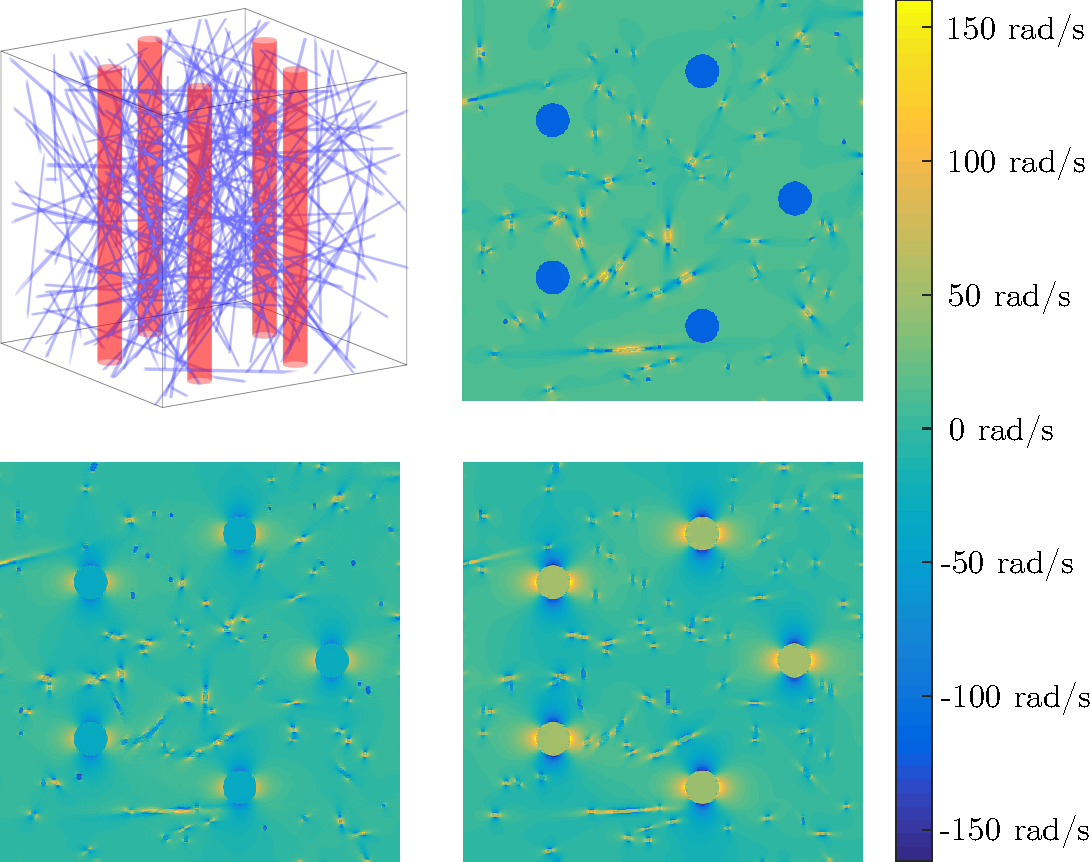
\includegraphics[keepaspectratio=true,width=\textwidth]{voxelgeo_domega_2x2}
    \caption{ The top-left figure shows an example voxel geometry.
      The $3\times 3\times \SI{3}{\milli\meter^3}$
      voxel is populated with an
      isotropic vascular bed and $L=5$ anisotropic large vessels in
      the $z$-direction. The total volume occupied by the blood
      vessels is determined by the blood volume fraction BVF. The
      relative fraction of blood contained in the isotropic vascular
      bed is determined by the isotropic relative blood volume
      fraction iRBVF, and the amount of blood contained in the
      anisotropic vessels is then $\text{aRBVF} = 1 - \text{iRBVF}$.
      The magnetic field generated by this configuration is computed
      by the convolution of the susceptibility map with the unit
      dipole kernel. Example cross-sections of the frequency shift
      map $\delta\omega$ are shown for $\alpha = 0\degree$ (top
      right), $45 \degree$ (bottom left), and $90 \degree$ (bottom
      right).  It can be easily observed that near large vessels, the
      resonance frequency (i.e. the magnetic field) remains locally
      relatively constant compared to the resonance frequency near
      small vessels, which changes rapidly over short distances.  Note
      also the increase in strength and range of inhomogeneities
      around the large anisotropic vessels as $\alpha$ increases,
      introducing the dependence on the angle $\alpha$ into the
      simulations.}
    \label{fig:geometry}
    \end{minipage}
\end{figure}

\clearpage
\begin{figure}[H]
\centering
\begin{minipage}{1.0\textwidth}

\centering
%\begin{minipage}{0.7\textwidth}
\begin{minipage}{1.0\textwidth}
\begin{algorithm}[H]
\setstretch{2.0}
\fontsize{16}{16}
\begin{algorithmic}[1]
    \algsetup{linenosize=\LARGE}
    \algsetup{indent=3em}
    \vspace{0.25cm}
    \STATE \text{\LARGE{}Initialize:} $\Mxy_0 \coloneqq i$,
    $\Delta t \coloneqq \text{TE}/30$, $k \coloneqq 0$

    \WHILE{ $k \Delta t < \text{TE}$ }
    
    \STATE $\Mxy_{k+\frac{1}{2}} \coloneqq 
    e^{-\CDecay(\vect{r}) \Delta t} \, \Mxy_k$
    %\COMMENT{$\Delta t \rightarrow \Delta t/2$}

    \STATE $\Mxy_{k+1} \coloneqq 
    \Phi(\vect{r},\Delta t) \conv \Mxy_{k+\frac{1}{2}}$
    %\COMMENT{$\Mxy_{k+1} \rightarrow \Mxy_{k+\frac{1}{2}}$}

    %\STATE \Comment{$\Mxy_{k+1} \coloneqq
    %e^{-\CDecay(\vect{r}) \Delta t/2} \Mxy_{k+\frac{1}{2}}$}

    \IF{ $(k+1) \Delta t = \text{TE}/2$ }
    \STATE $\Mxy_{k+1} \coloneqq \conj{\Mxy}_{k+1}$
    \ENDIF
    
    \STATE $k \coloneqq k + 1$
    
    \ENDWHILE
    
    \STATE $S(\text{TE}) \coloneqq \int \Mxy_k \, d^3\vect{r}$
\end{algorithmic}
\captionsetup{strut=off}
\caption*{\Large{}\textbf{Magnetization Propagation Algorithm}}
\end{algorithm}
\end{minipage}

%\captionsetup{font=small,skip=0pt}
\addtocounter{figure}{-1} %Want this to be labelled as the first Algorithm
\renewcommand{\figurename}{Algorithm}
\caption{Magnetization propagation algorithm used to simulate the signal
    $S(\text{TE})$ for a given set of free parameters 
    $\text{CA}_{\text{PEAK}}$, BVF, iBVF, and $L$. 
    All four free parameters are encoded solely in the complex decay rate 
    $\CDecay(\vect{r})$; the rest of the algorithm does not depend on them.
    The notation $\Mxy_\nu$ is shorthand for 
    $\Mxy(\vect{r},\nu \Delta t)$ throughout the algorithm.
    If the $\mathcal{O}(\Delta t^3)$ order evolution 
    equation \ref{EvolSplit_Order3} were used instead,
    line 3 should be modified to decay for only a half time step $\Delta t/2$,
    line 4 should perform the Gaussian convolution in-place,
    and an extra line should be added directly following the convolution which
    decays for another half time step $\Delta t/2$.}
    \label{fig:algorithm1}
\end{minipage}
\end{figure}

\clearpage
\begin{figure}[H]
\centering
\begin{minipage}{1.0\textwidth}
    \centering
    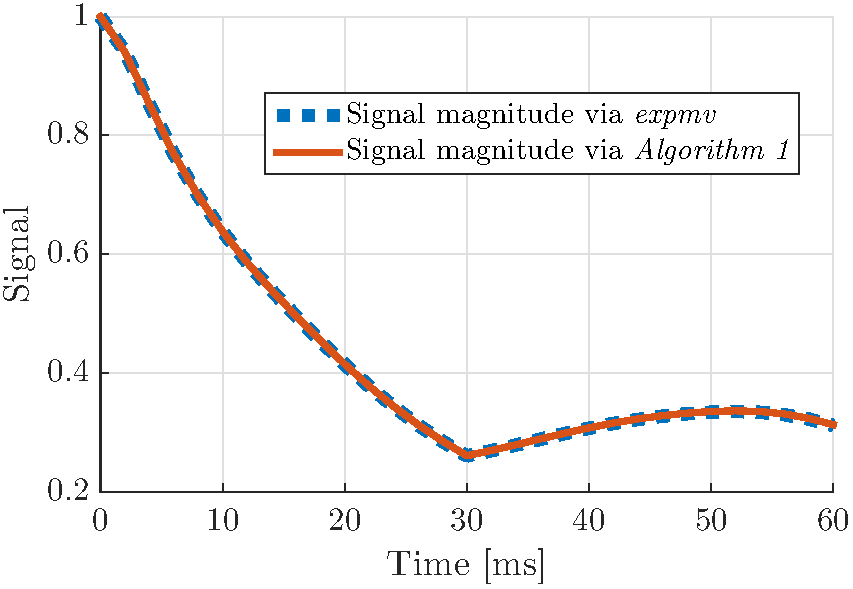
\includegraphics[keepaspectratio=true,width=1.0\textwidth]{SE_Signal_vs_Time_ConvDiff_vs_Expmv}
    \caption{Comparison between solving the Bloch-Torrey equation
          exactly using the method of lines in conjunction with
          Higham's \textit{expmv}
          integrator~\cite{al-mohy_computing_2011}, and solving the
          Bloch-Torrey equation approximately using the two-step
          approximate solution as described in
          Algorithm~\ref{fig:algorithm1}. The signal decay through
          time calculation shows strong agreement between the two
          methods, with error values of 0.064\% +/- 0.045\%; the
          maximum error value of 0.14\% occurs at $\unit[60]{ms}$.}
    \label{fig:comparison}
\end{minipage}
\end{figure}

\clearpage
\begin{figure}[H]
\centering
\begin{minipage}{1.0\textwidth}
    \centering
    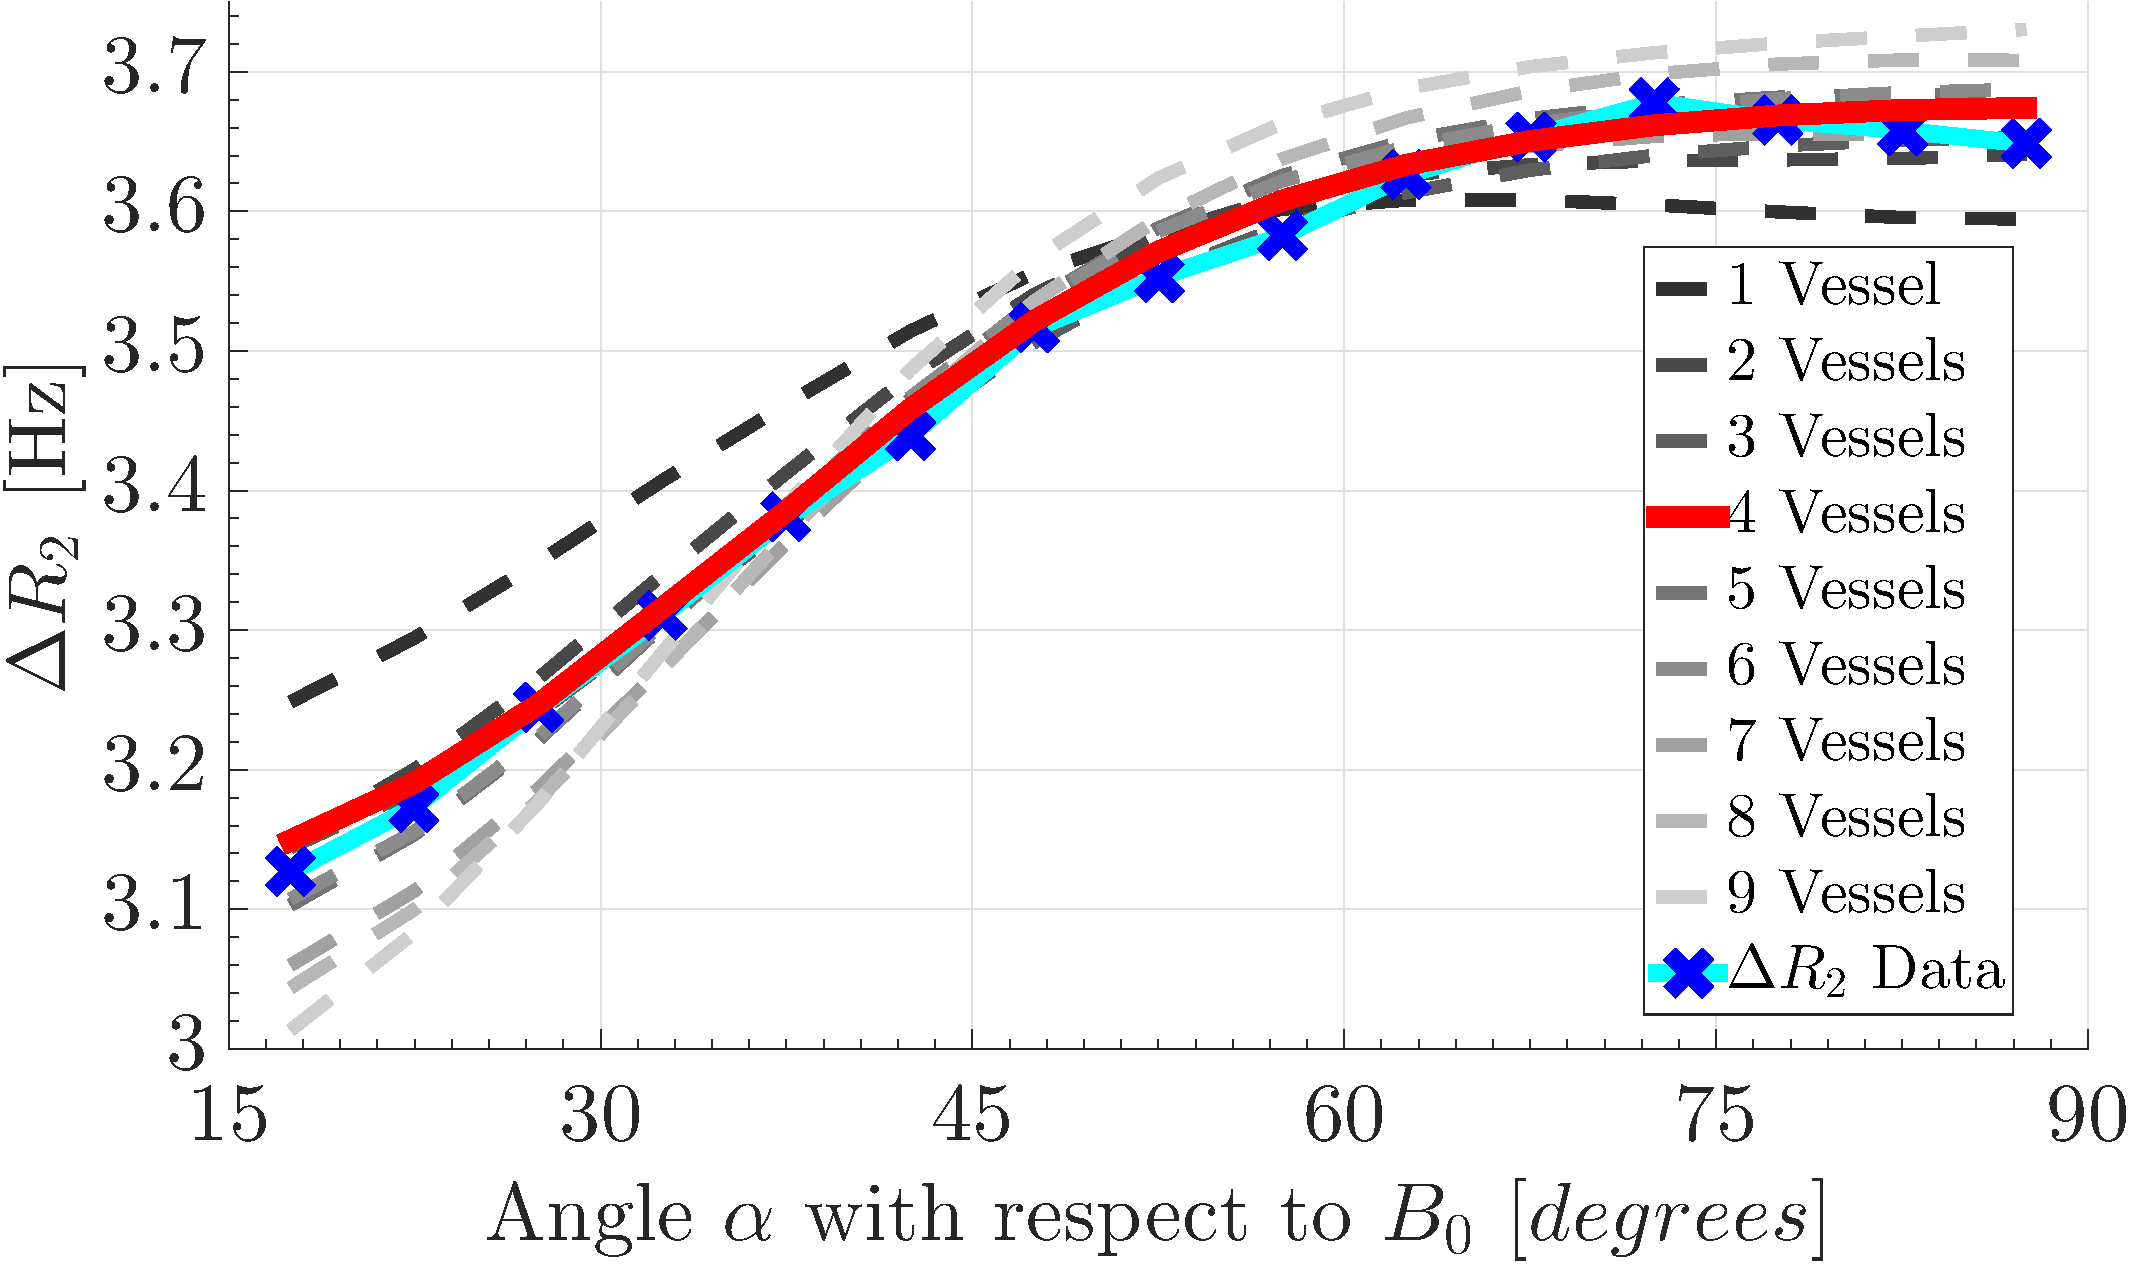
\includegraphics[keepaspectratio=true,width=1.0\textwidth]{Combined_SimulationVsData_4Major_Highlighted_7umMinor}
    \caption{$\Delta R_2$ vs.\@ $\alpha$ (blue) and fitted model
          (red) for $L$ = \Lbest{} anisotropic blood vessels.
          $\Delta R_2$ was 20\% larger for fibres perpendicular
          to the main magnetic field compared to parallel fibres.
          The resulting parameters found are
          $\text{CA}_{\text{PEAK}}$ = \CAbest{},
          BVF = \BVFbest{}, and iRBVF = \iRBVFbest{},
          corresponding to \iBVFbest{} of cerebral blood in
          isotropic vasculature and \aBVFbest{} in anisotropic
          vasculature. It should be noted that >97\% of data points
          have an angle with $B_0$ greater than 15°. For angles below
          15°, there was an upward trend that may be an artifact
          of the small number of voxels contributing to these angles.
          This trend was not observed in the gradient echo EPI
          experiment~\cite{hernandez-torres_anisotropic_2016},
          nor in the simulations of this study,
          and therefore these points were excluded for the
          purposes of parameter fitting.}
    \label{fig:dR2curves}
\end{minipage}
\end{figure}

%\clearpage
%\begin{figure}[H]
%\centering
%\begin{minipage}{1.0\textwidth}
%    \centering
%    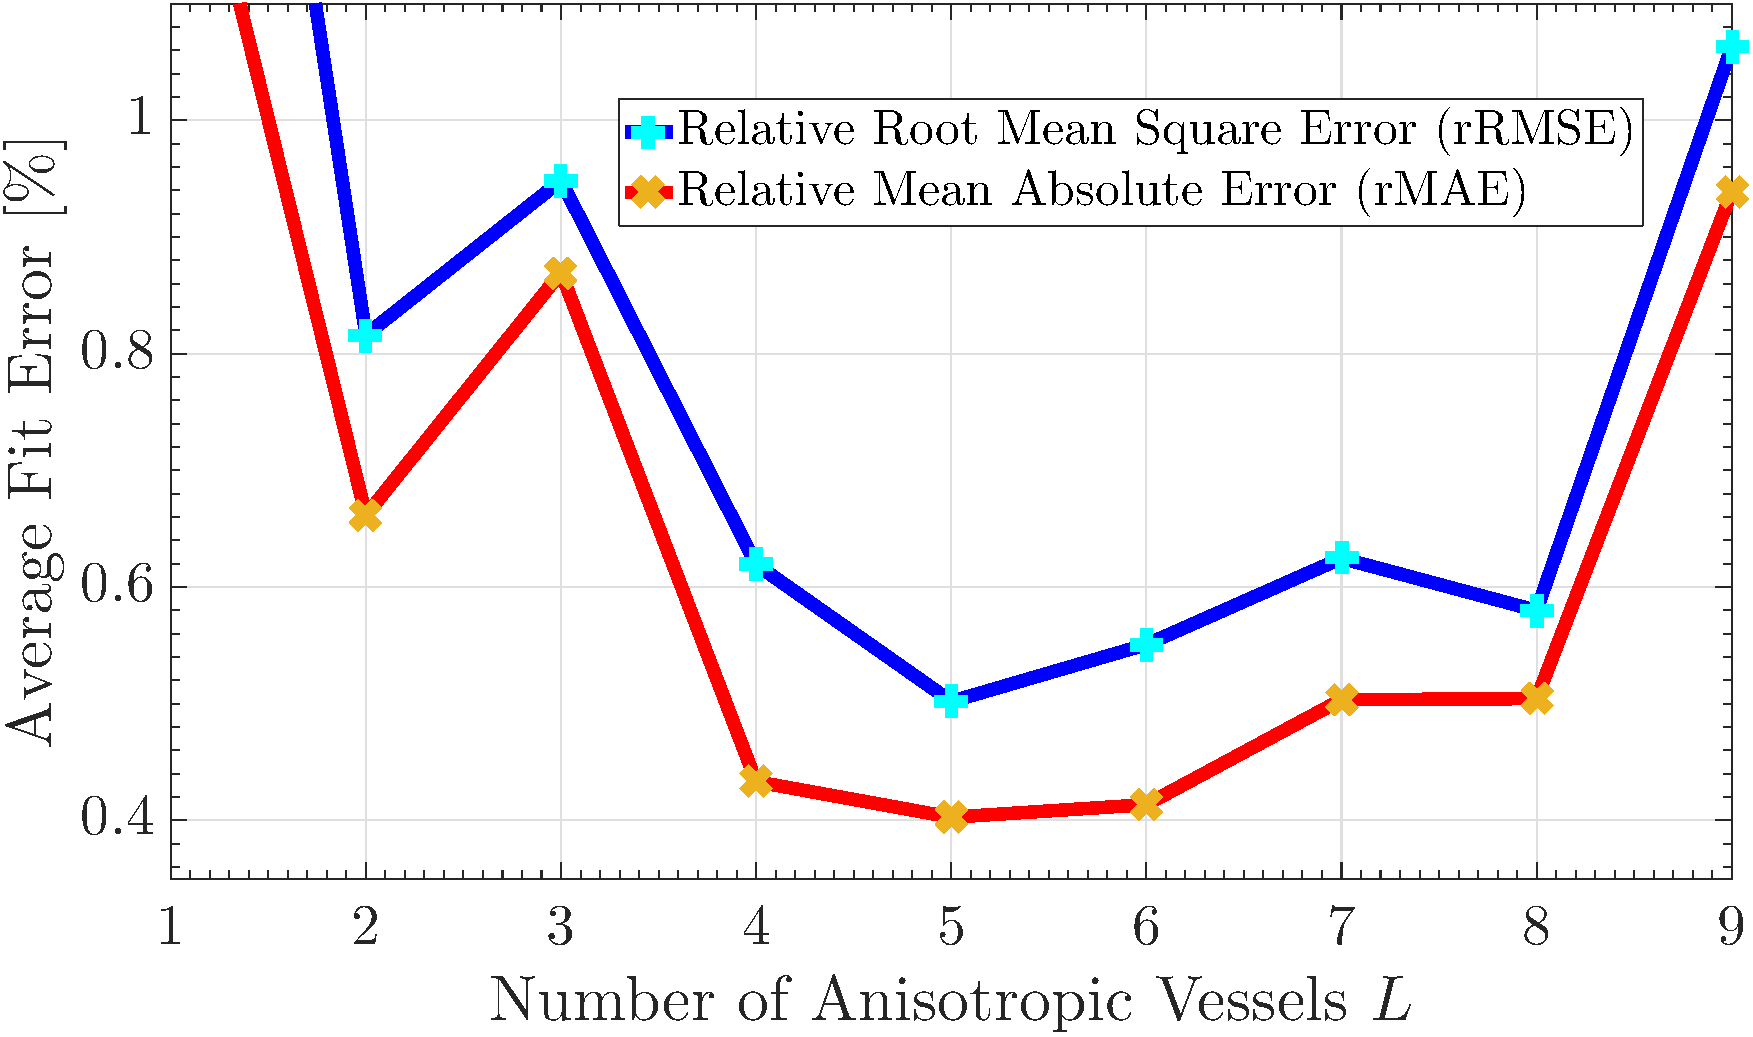
\includegraphics[keepaspectratio=true,width=1.0\textwidth]{ErrorPlot_Combined_SimulationVsData_v2}
%    \caption{Plot of the error in the best fit model versus the
%          number of anisotropic vessels. The relative root mean
%          square error and the relative mean absolute error are both
%          calculated relative to the mean of the $\Delta R_2$ data
%          set. For both error metrics, the lowest error was obtained
%          from the model using $L=5$ anisotropic blood vessels.}
%    \label{fig:errorcurves}
%\end{minipage}
%\end{figure}

\clearpage
\begin{figure}[H]
\centering
\begin{minipage}{1.0\textwidth}
    \centering
    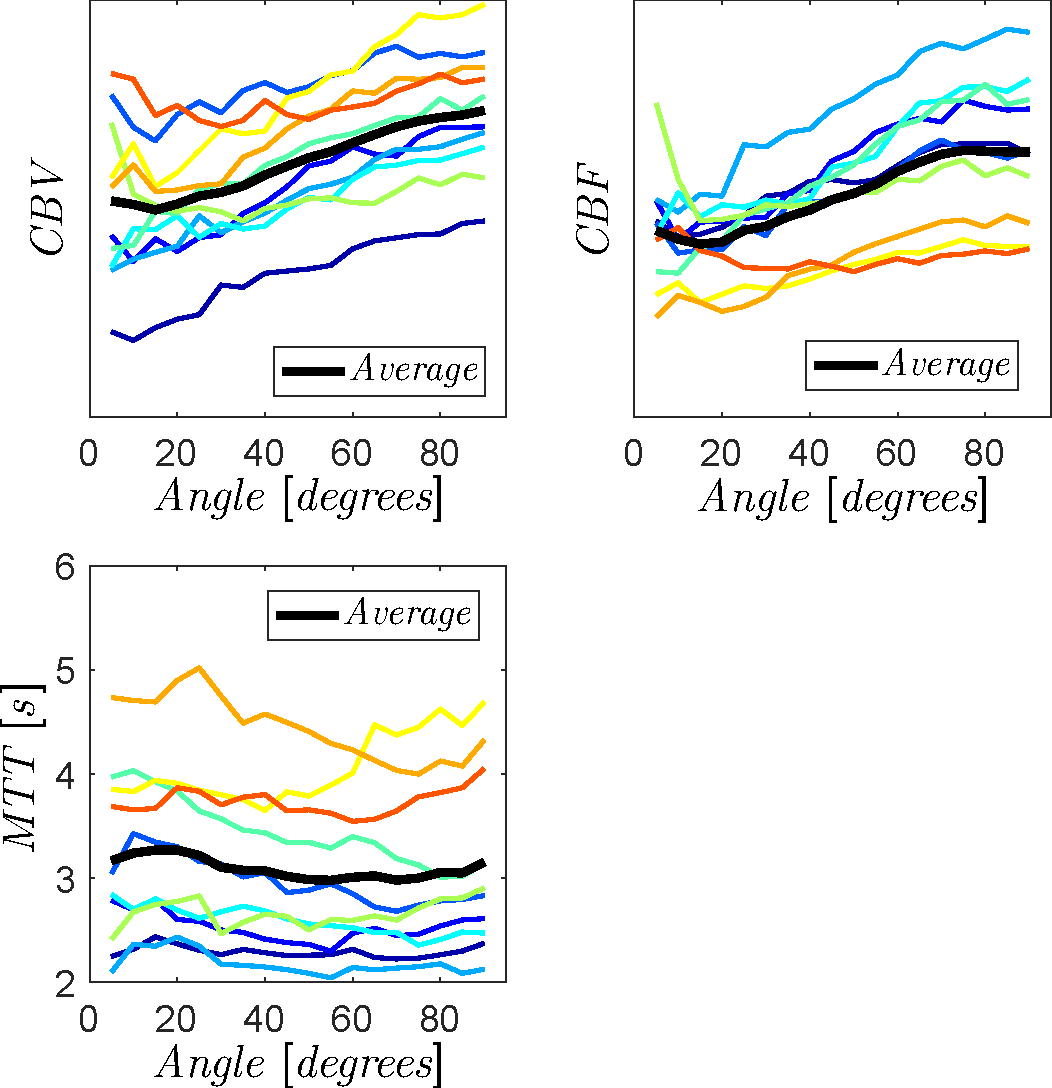
\includegraphics[keepaspectratio=true,width=0.9\textwidth]{angle_dependence_CBF_CVV_MTT_spin_echo_NEW_cropped}
    \caption{CBV and CBF exhibit larger values at 90$\degree$
          compared to 0$\degree$. The orientation dependence of MTT is
          weak. Coloured curves represent individual subjects.
          As no normalization of CBV and CBV to an internal
          reference tissue was performed, both CBV and CBF are given
          in arbitrary units, which were normalized to the average from
          zero to five degrees.}
    \label{fig:perfusioncurves}
\end{minipage}
\end{figure}

\clearpage
\begin{figure}[H]
\centering
\begin{minipage}{1.0\textwidth}
    \centering
    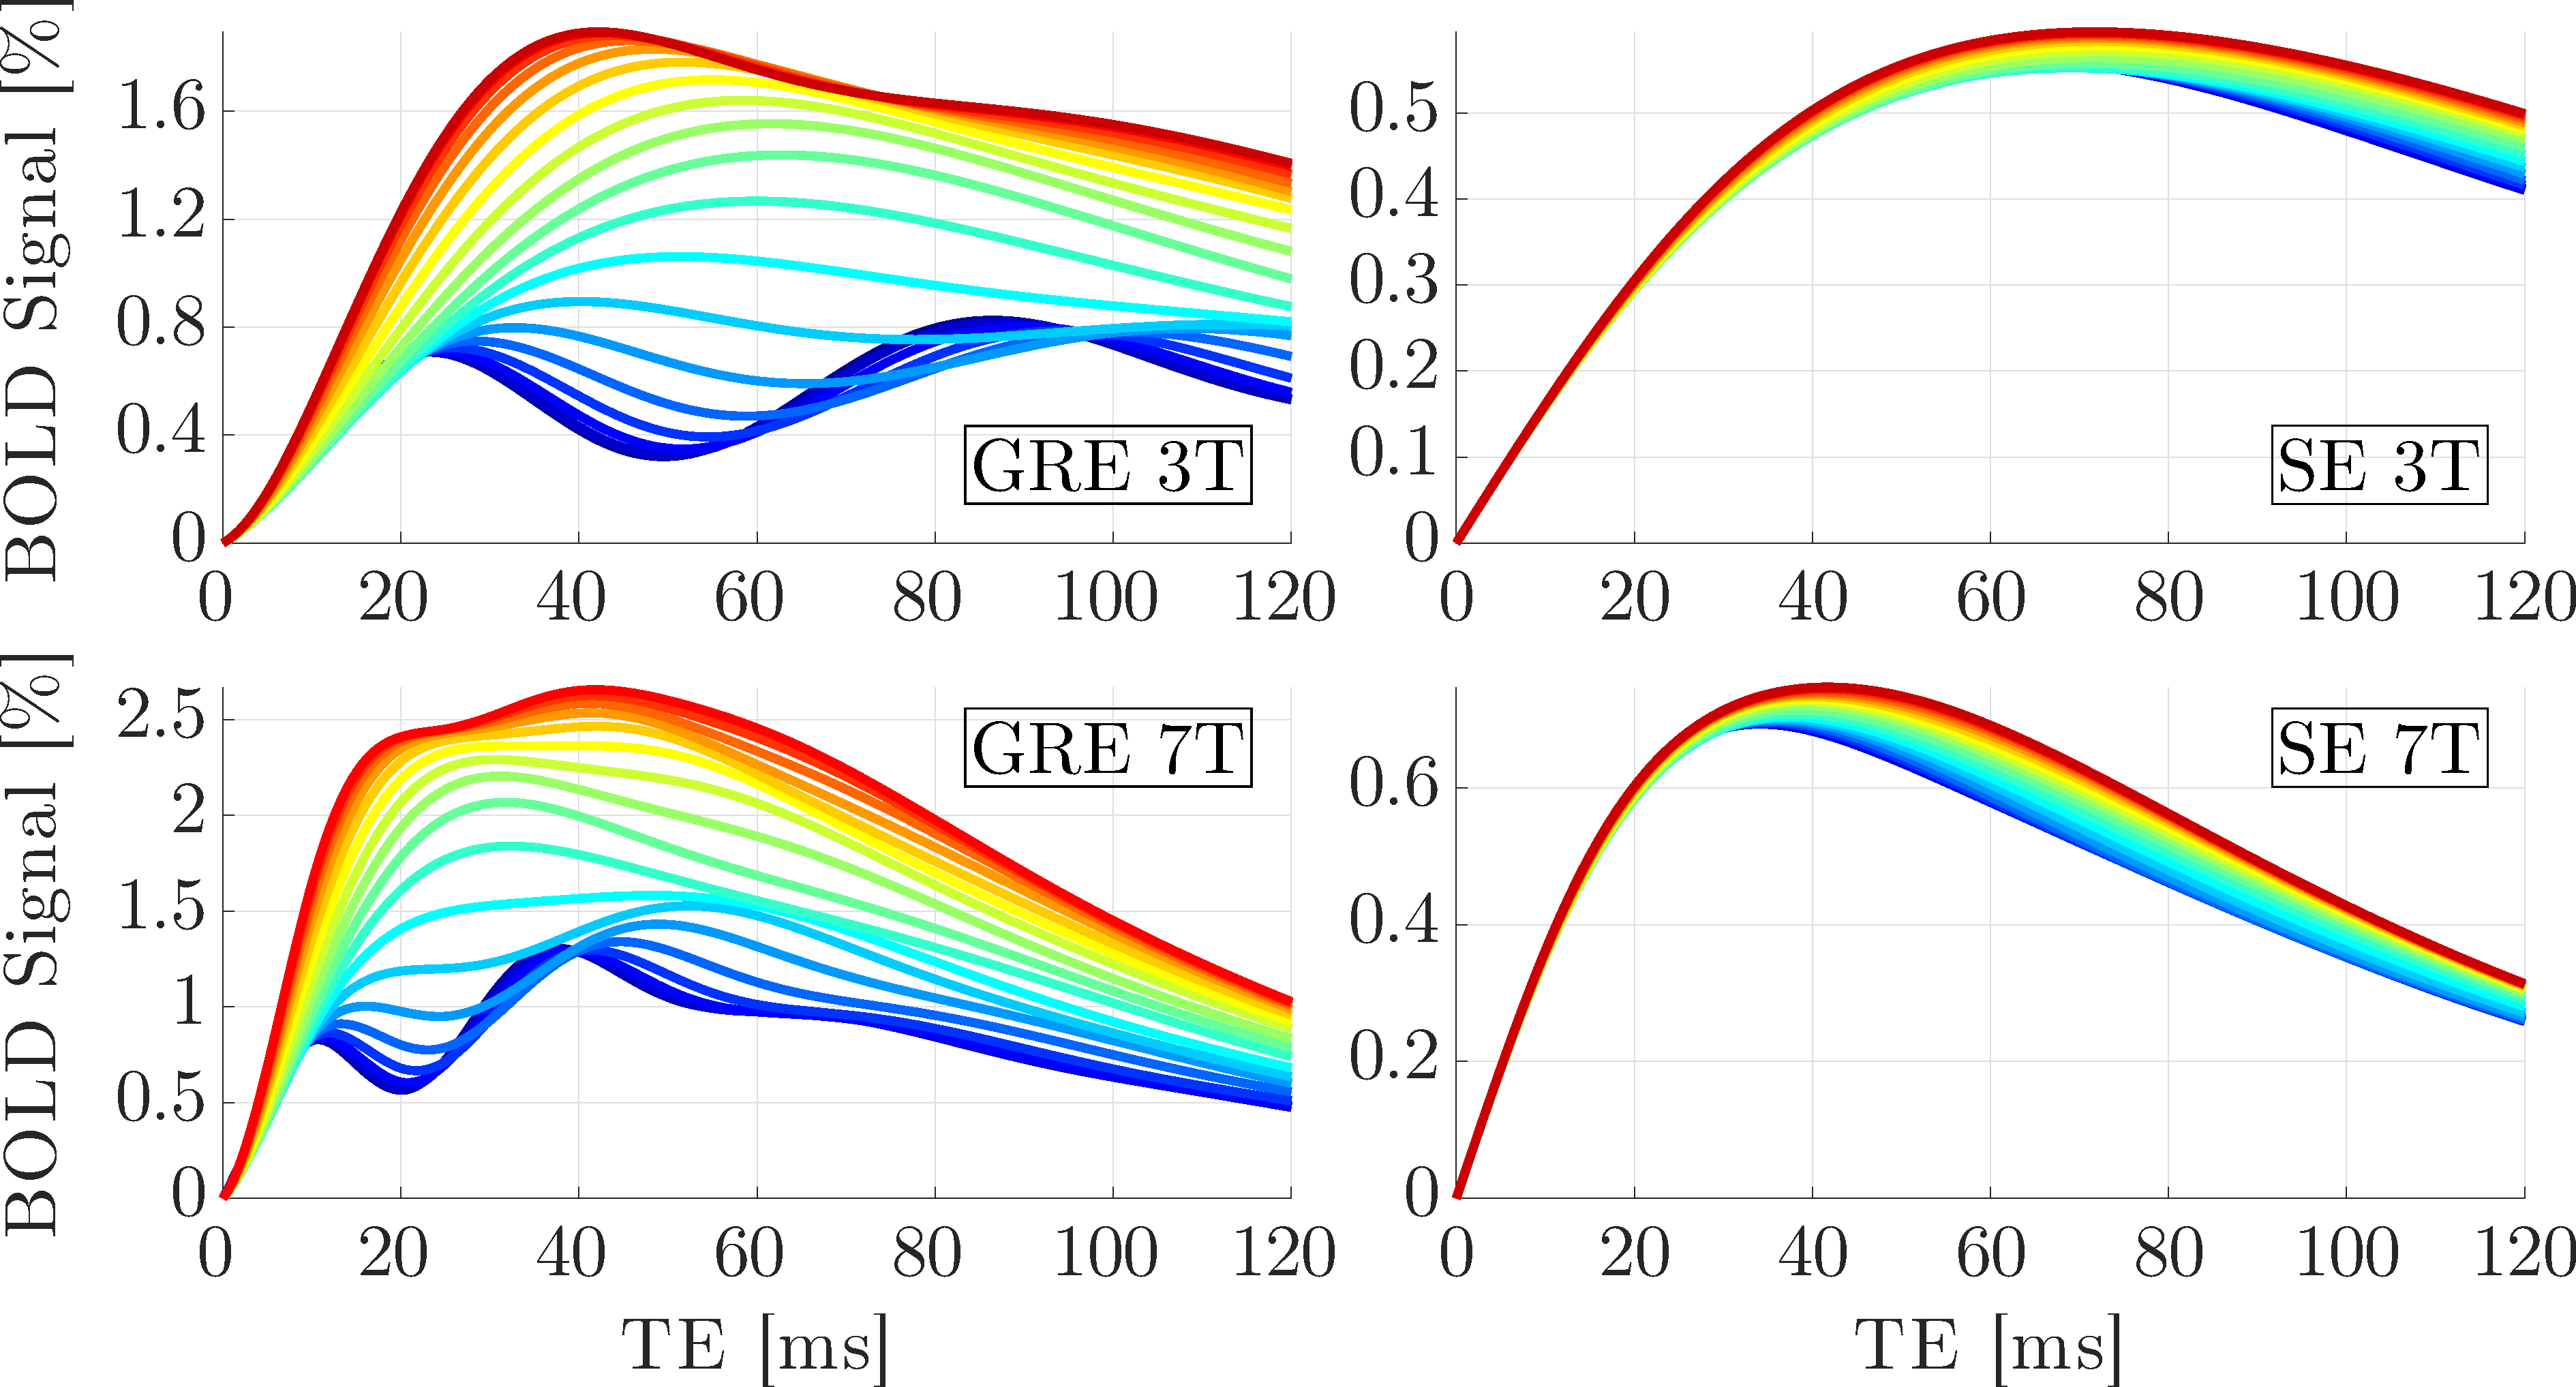
\includegraphics[keepaspectratio=true,width=1.0\textwidth]{BOLDPlots_7umMinor_ThirdArteries}
    \caption{The WM BOLD signal for gradient echo (left) and
    spin echo (right) fMRI at $\unit[3]{T}$ (top) and $\unit[7]{T}$ (bottom).
    The gradient echo signal exhibits a strong angle dependence of up to
    100\% for for echo times between 25 and $\unit[60]{ms}$, whereas in
    the spin echo angle dependence does not exceed 20\%. Since the
    spin echo angle dependence is diffusion mediated, it does not
    become relevant until $\unit[40]{ms}$. The colours represent
    fibre orientations ranging from
    \SI{0}{\degree} (dark blue) to \SI{90}{\degree} (dark red).
    Note that the BOLD contrasts are not scaled for field strength.}
    \label{fig:BOLD}
\end{minipage}
\end{figure}

\clearpage
\setcounter{page}{1}
\setcounter{figure}{0}
\renewcommand{\thepage}{S\arabic{page}}
\renewcommand{\thesection}{S\arabic{section}}
\renewcommand{\thetable}{S\arabic{table}}
\renewcommand{\thefigure}{S\arabic{figure}}
\section*{Supplemental Materials}
% ---- Supplemental Text ---- %
%\subsection*{Supplemental Text}
Using MR vessel size imaging, Jochimsen and colleagues reported radii of \SI{13.7}{\micro\meter} with a standard deviation of \SI{2.1}{\micro\meter}~\cite{jochimsen_whole-brain_2010}.
Additional experiments were performed with these parameters to see what effects doubling of the capillary radius has on the results.
All other factors held constant, the fit to the perfusion orientation experiment was performed to determine vascular parameters, followed by the simulated BOLD experiment, as was done for the case of the smaller \SI{7}{\micro\meter} radius minor vasculature and described in the manuscript.

The results of the fit to the perfusion experiment in Figure~\ref{fig:S1-PerfOrientation} illustrate the robustness of the fit parameters to changes in vessel sizing.
While the total blood volume fraction BVF increases, the increase is almost entirely due to increased isotropic blood (from \iBVFbest{} to 2.30\%).
The anisotropic blood fraction decreases slightly from \aBVFbest{} to 1.19\%.

This increase in isotropic blood volume is expected due to the fact that diffusion mediated spin dephasing is sensitive to local magnetic field gradients, which are weaker in the case of larger minor vessels.
This results in a larger fraction of blood being required to produce the same (orientation independent-) change in $R_2$ when compared to isotropic vasculature that consists of smaller vessels.

The differing anisotropic blood volume fractions is partly due to the differing number of optimal vessels L.
In fact, the optimal anisotropic BVF for the \SI{7}{\micro\meter} experiment corresponding to $L=5$ was 1.28\%.
The anisotropic BVF is therefore relatively independent of the minor vasculature, as is expected  when the cause of the orientation dependency is strictly due to the anisotropic blood, and not the isotropic blood.
Note that the total blood volume computed with \SI{7}{\micro\meter} experiment (\BVFbest{}) is very close to the blood volume determined with positron emission tomography (2.6\%), whereas the \SI{13.7}{\micro\meter} experiment results in a blood volume that is much larger at 3.5\%.

The remaining variable parameter, the contrast agent concentration, was relatively independent of minor vessel size as well.
The \SI{7}{\micro\meter} experiment found CA values of \CAbest{} for L = 4 anisotropic vessels and \SI{6.30}{\milli\Molar} for L = 5 vessels, compared with \SI{6.23}{\milli\Molar} for L = 5 vessels for the 13.7 \SI{}{\micro\meter} experiment.

Lastly, the strength and orientation of the BOLD signals in Figure~\ref{fig:S2-BOLDPlots} calculated at 3T and 7T for SE and GRE scans were consistent as well.
The peak strength of the BOLD signals all decreased approximately proportional to the change in total BVF (\BVFbest{}/3.49\% = 0.722, or roughly two-thirds to three-quarters).
The orientation dependency of the SE BOLD signal is the same as in the \SI{7}{\micro\meter} experiment; the GRE BOLD signal orientation dependency is weaker. 

In summary, the parameters of interest (anisotropic blood volume and the BOLD effect) are relatively insensitive to changes in microvascular parameters.

\clearpage
\subsection*{Supplemental Figures}
% ---- Supplemental Figures ---- %

\begin{figure}[H]
\centering
\begin{minipage}{1.0\textwidth}
    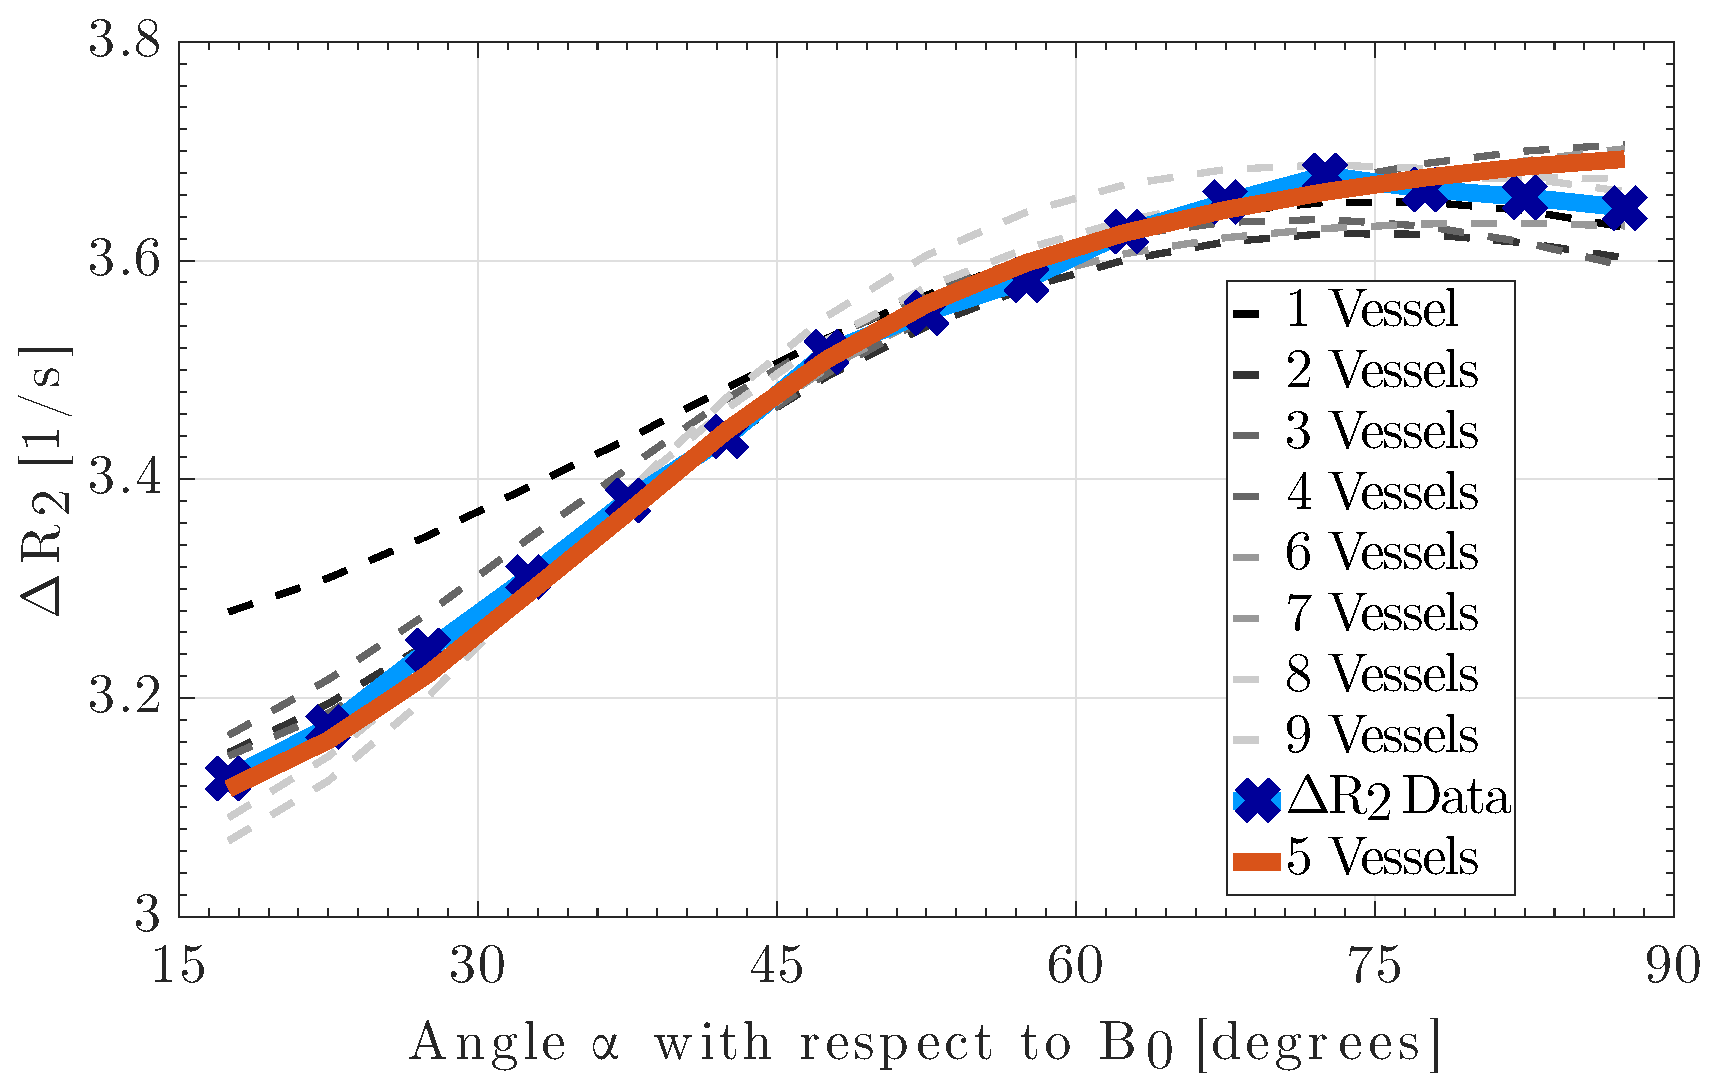
\includegraphics[keepaspectratio=true,width=1.0\linewidth]{supplemental_figures/Figure_S1--Combined_SimulationVsData_5Major_Highlighted_v3}
    \caption{$\Delta R_2$ vs.\@ $\alpha$ (blue) and fitted model (red) for $L = 5$ anisotropic blood vessels.
    $\Delta R_2$ was 20\% larger for fibres perpendicular to the main magnetic field compared to parallel fibres.
    The resulting parameters found are $\text{CA}_{\text{PEAK}}$ = \SI{6.23}{\milli\Molar}, BVF = 3.49\%, and iRBVF = 65.9\%, corresponding to 2.30\% of cerebral blood in isotropic vasculature and 1.19\% in anisotropic vasculature.
    It should be noted that >97\% of data points have an angle with $B_0$ greater than \SI{15}{\degree}.
    For angles below \SI{15}{\degree}, there was an upward trend that may be an artifact of the small number of voxels contributing to these angles.
    This trend was not observed in the gradient echo EPI experiment~\cite{hernandez-torres_anisotropic_2016}, nor in the simulations of this study, and therefore these points were excluded for the purposes of parameter fitting.}
    \label{fig:S1-PerfOrientation}
\end{minipage}
\end{figure}

\clearpage
\begin{figure}[H]
\centering
\begin{minipage}{1.0\textwidth}
    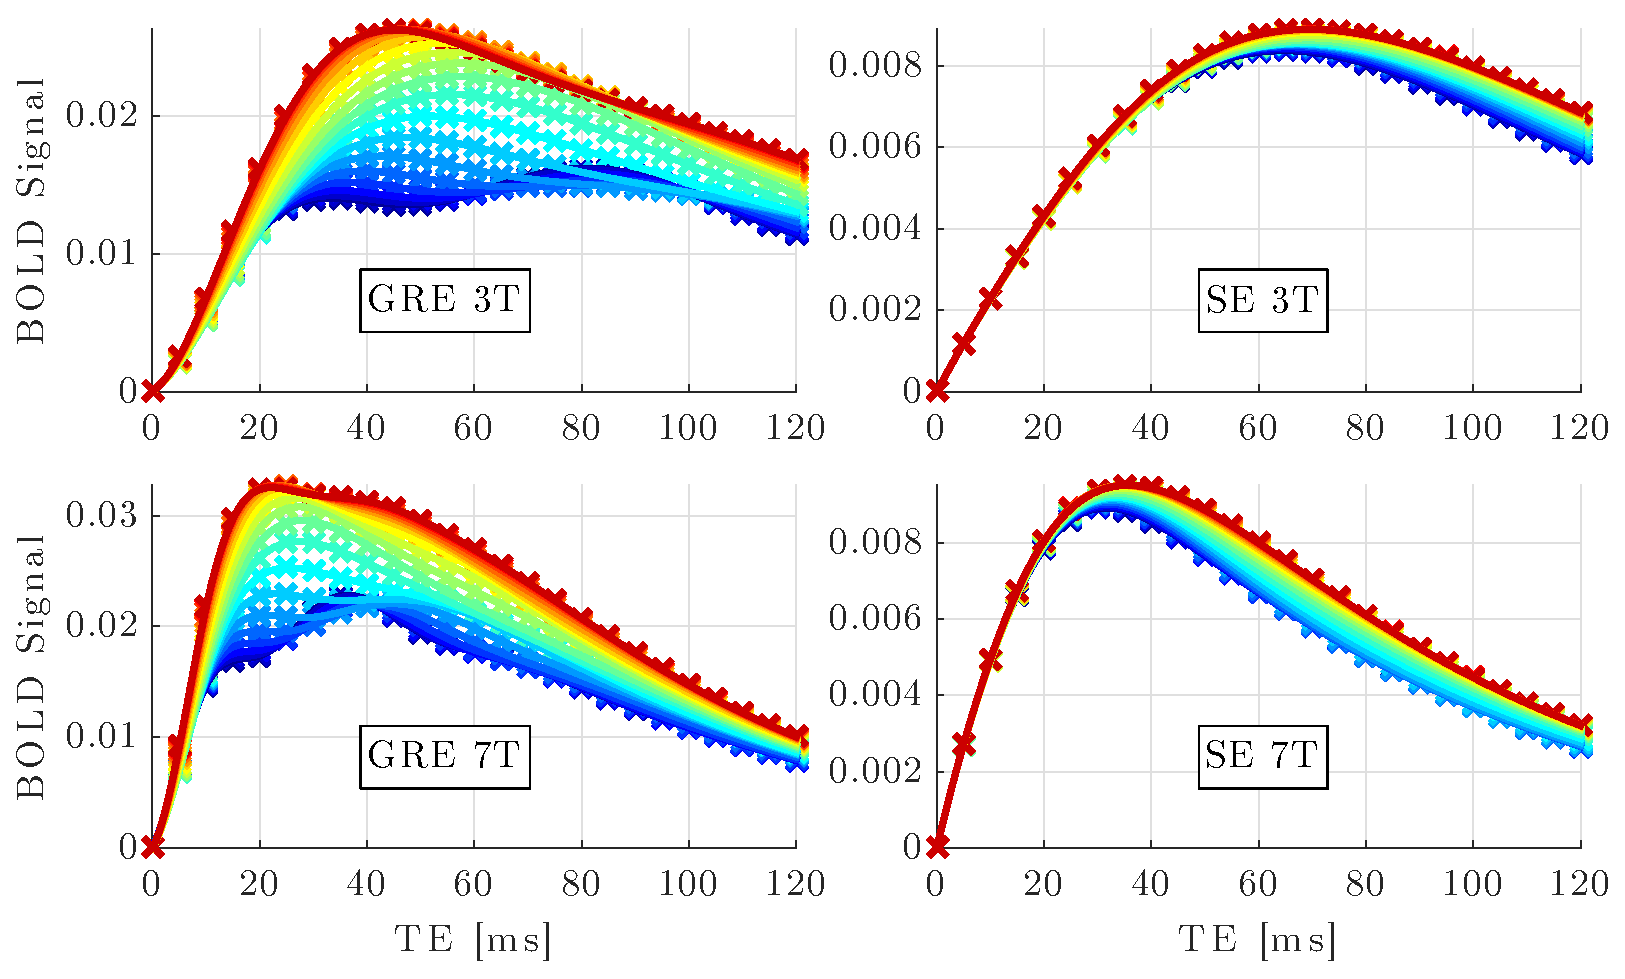
\includegraphics[keepaspectratio=true,width=1.0\linewidth]{supplemental_figures/Figure_S2--BOLDPlots_075_BVF_mod3}
    \caption{The WM BOLD signal for gradient echo (left) and spin echo (right) fMRI at 3T (top) and 7T (bottom).
    The gradient echo signal exhibits a strong angle dependence of up to 100\% for for echo times between 25 and \SI{60}{\milli\second}, whereas in the spin echo angle dependence does not exceed 20\%.
    Since the spin echo angle dependence is diffusion mediated, it does not become relevant until \SI{40}{\milli\second}.
    The colours represent fibre orientations ranging from \SI{0}{\degree} (dark blue) to \SI{90}{\degree} (dark red).
    Note that the BOLD contrasts are not scaled for field strength.}
    \label{fig:S2-BOLDPlots}
\end{minipage}
\end{figure}

% ---- Supplemental figures for review only ---- %
\clearpage
\subsection*{Supplemental Figures For Review Only}
\renewcommand{\thefigure}{S\arabic{figure}, For Review Only}

\begin{figure}[H]
\centering
\begin{minipage}{1.0\textwidth}
    \centering
    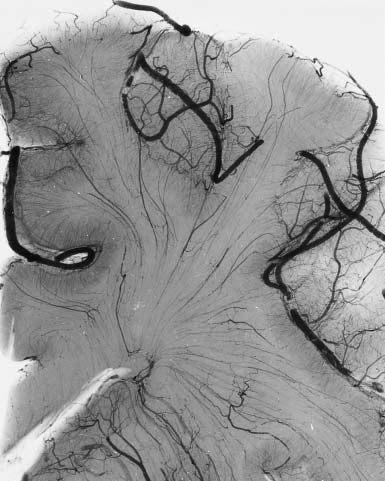
\includegraphics[keepaspectratio=true,width=0.85\textwidth]{supplemental_figures/Figure_S3--Nonaka_et_al_2003--Cerebral_Hemisphere_Soft_Xray}
    \caption{Soft X-ray picture of the cerebral hemisphere.
    Many arterial branches terminate in the cortex and subcortical white matter.
    Some large arteries run in straight lines centripetally toward the lateral ventricle.
    No centrifugal arteries are noted.
    \textbf{(This figure and its capture were taken from Nonaka et al. Neuropathology 2003, 23, 111-118~\cite{nonaka_microvasculature_2003}}.)}
    \label{fig:S3-CerebSoftXray}
\end{minipage}
\end{figure}

\clearpage
\begin{figure}[H]
\centering
\begin{minipage}{1.0\textwidth}
    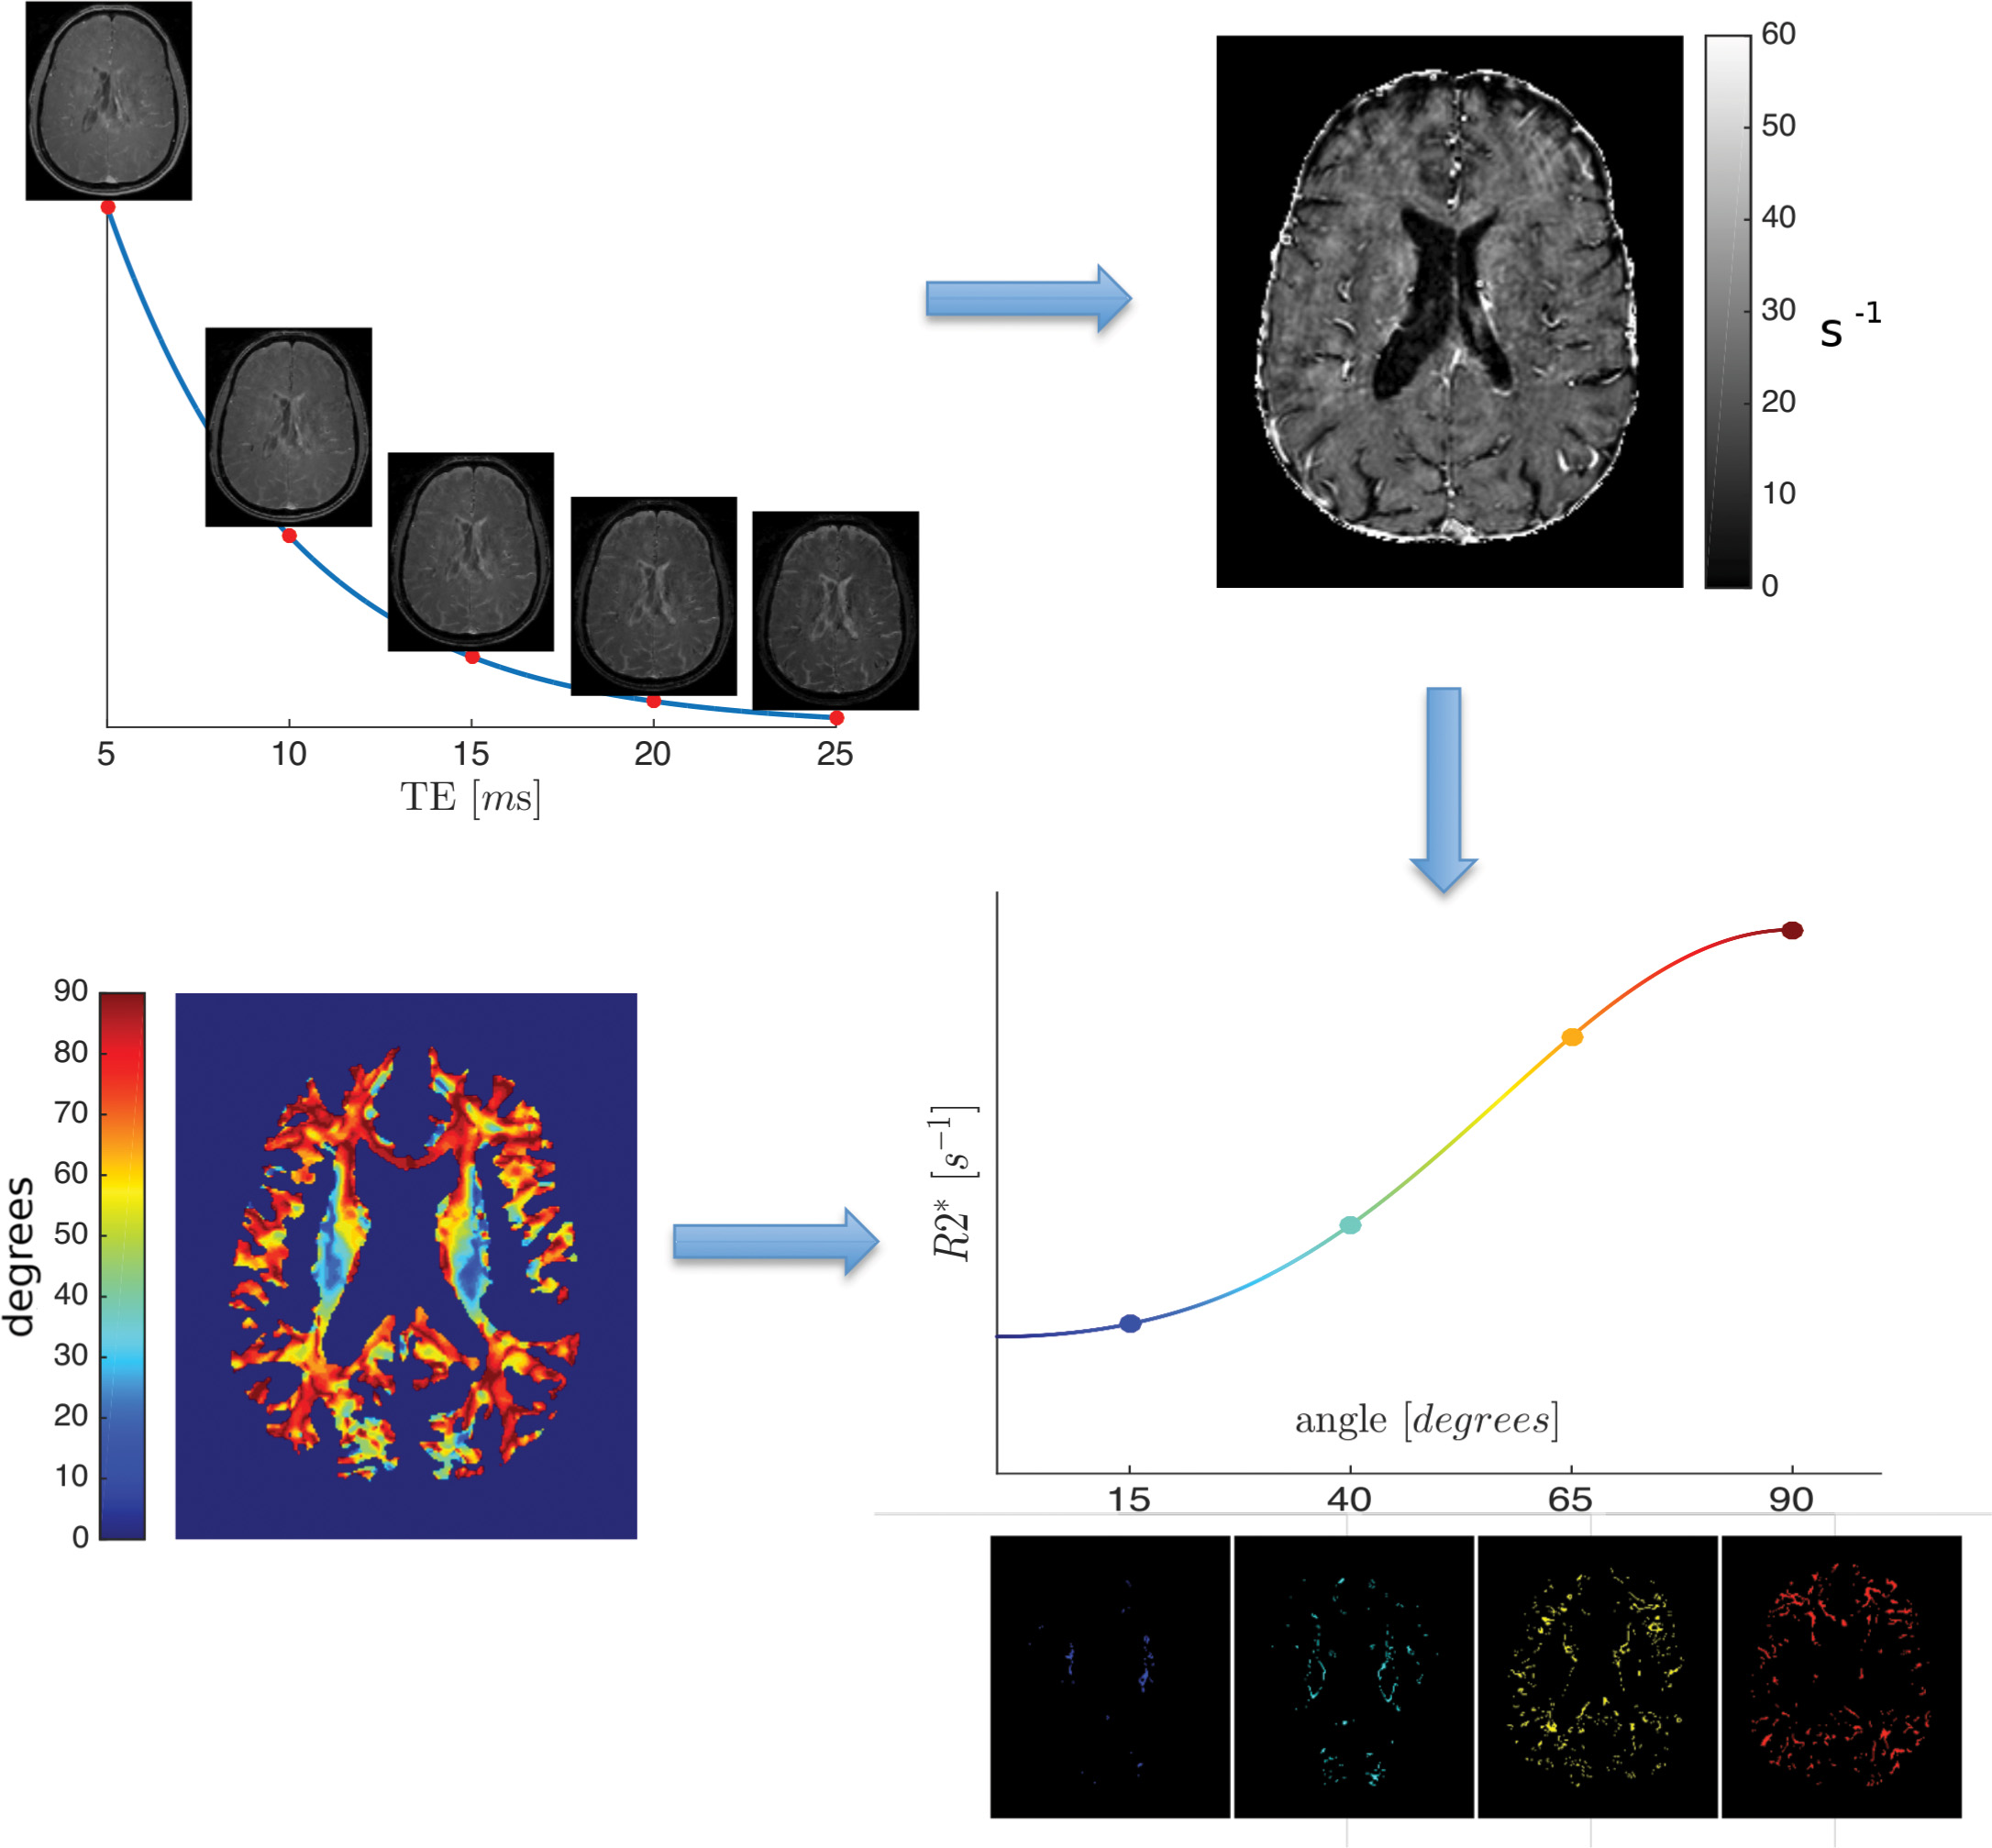
\includegraphics[keepaspectratio=true,width=1.0\linewidth]{supplemental_figures/Figure_S4--Hernandez-Torres_et_al_2015--Orientation_Mapping_Workflow}
    \caption{Data processing workflow for orientation mapping.
    The angle between the largest eigenvector of the diffusion tensor and $B_0$ is computed in each voxel.
    The quantitative image values (in this image it is $R_2^*$; for the present perfusion data it is $\Delta R_2$) from each orientation interval are pooled together, averaged and then plotted against the corresponding orientation.
    The four exemplary images below the $R_2^*$ curve represent four angle intervals (10–15, 35–40, 60–65, and 85–90 degrees, respectively) and show which voxels contribute to the $R_2^*$ average.
    Their color corresponds to the color of the angle map.
    \textbf{(Image taken from Hernández-Torres, \dots, Rauscher: PLOS ONE 2015.)}}
    \label{fig:S4-OrientMapping}
\end{minipage}
\end{figure}

\clearpage
\begin{figure}[H]
\centering
\begin{minipage}{1.0\textwidth}
    \centering
    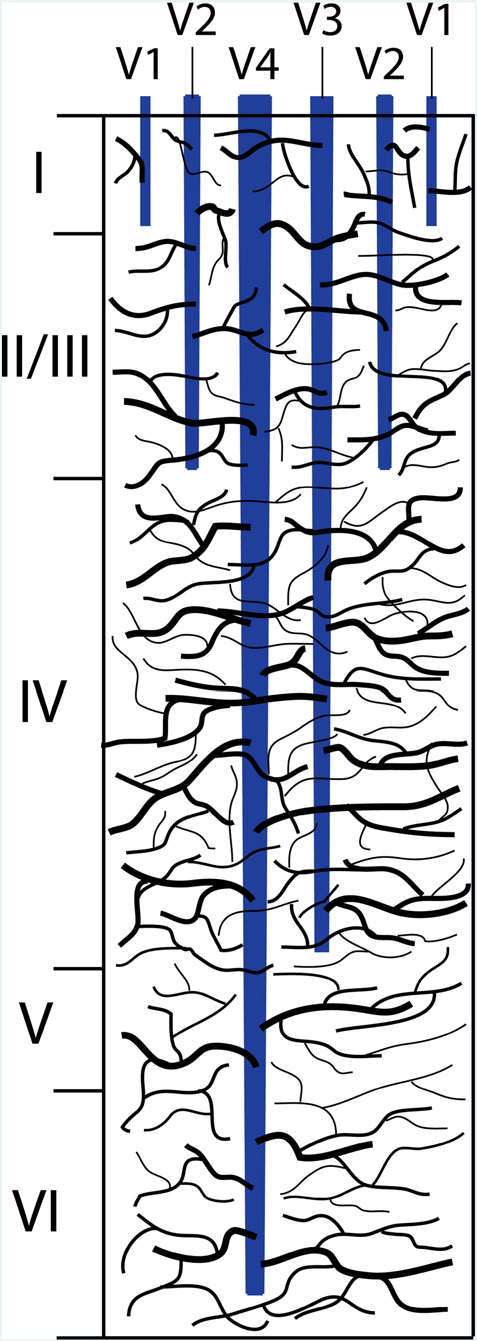
\includegraphics[keepaspectratio=true,width=0.4\linewidth]{supplemental_figures/Figure_S5--Markuerkiaga_et_al_2016--Cortical_Levels}
    \caption{Figure~1 from Markuerkiaga, Barth \& Norris, Neuroimage 2016~\cite{markuerkiaga_cortical_2016}, showing different calibers of cortical veins at different cortical levels.
    See also Duvernoy, Delon, Vannson 1981~\cite{duvernoy1981}.}
    \label{fig:S5-CorticalLevels}
\end{minipage}
\end{figure}

\end{document}
